\documentclass[12pt, a4paper]{article}

\usepackage{fancyhdr}
\usepackage[left=4cm, right=4cm, top=4cm, bottom=4cm]{geometry}
\usepackage[utf8]{inputenc}
\usepackage[table]{xcolor}
\usepackage{amsmath}
\usepackage{enumitem}
\usepackage{graphicx}
\usepackage{hyperref}
\usepackage{geometry}
\usepackage{booktabs}
\usepackage{algpseudocode}
\usepackage[ruled,linesnumbered]{algorithm2e}
\usepackage{subcaption}
\usepackage{xepersian}

\DeclareMathOperator*{\argmax}{argmax}
\DeclareMathOperator*{\argmin}{argmin}
\newcolumntype{L}{>{$}l<{$}} % math-mode version of "l" column type

\newcommand{\coursetitle}{شناسایی آماری الگو}
\newcommand{\doctitle}{پروژه پایان‌ترم}
\newcommand{\name}{محمدرضا غفرانی}
\newcommand{\studentno}{400131076}
\newcommand{\todaydate}{\today}

\settextfont{Sahel}
\setlatintextfont{Times Newer Roman}

\pagestyle{fancy}
\lhead{\textbf{\doctitle}}
\chead{\name}
\rhead{\todaydate}

\begin{document}

\begin{flushleft}
    \name \\
    \studentno \\
    \todaydate
\end{flushleft}

\begin{center}
    \huge
    \textbf{\coursetitle}
    \break
    \large
    \doctitle
\end{center}

% suppress the fancy header on the first page only
\thispagestyle{plain}

\noindent

\section*{مقاله اول}

\begin{table}[h]
    \centering
    \caption{جدول مشخصات مقاله اول}
    \begin{tabular}{c|p{.7\linewidth}}
        مشخصه & توضیح \\
        \hline
        عنوان مقاله & \lr{Deep feature weighting for naive Bayes and its application to text classification} \\
        سال انتشار & 2016 \\
    \end{tabular}
\end{table}

روش \lr{naive Bayes} یکی از پراستفاده‌ترین روش‌ها برای حل مسائل دسته‌بندی در حوزه هوش مصنوعی است.
این روش علی‌رغم پرکاربرد بودن، فرض محدودکننده‌ای دارد و آن مستقل فرض کردن ویژگی‌ها از یکدیگر است.
با توجه به عملکرد بسیار خوب این روش علی‌رغم محدودیت‌های آن، محققان مختلف
سعی کرده‌اند راه‌هایی برای بهبود این روش بیابند. راهکارهای ارائه شده در دسته‌های زیر قرار می‌گیرند.

\begin{itemize}
    \item گسترش ساختار\LTRfootnote{structure extension}: در این روش با دستکاری و گسترش ساختار \lr{naive Bayes}
    تلاش می‌شود، وابستگی بین ویژگی‌ها بیشتر مشخص شود.
    \item انتخاب ویژگی‌\LTRfootnote{feature selection}: در این روش‌ها با انتخاب ویژگی‌های بهینه و حذف ویژگی‌های
    بی‌اهمیت، تلاش می‌شود با مقابله با معضل بعد\LTRfootnote{curse of dimensionality}، عملکرد الگوریتم بهتر شود.
    \item وزن‌دهی به ویژگی‌ها\LTRfootnote{feature weighting}: در این روش‌ها به جای حذف ویژگی‌های بی‌اهمیت، به آن‌ها
    وزن کم‌تری نسبت به ویژگی‌های بهینه داده شده و بدین طریق تلاش می‌شود تا ویژگی‌های بهینه تاثیر بیشتری در
    تصمیم اتخاذ شده داشته باشند.
    \item انتخاب نمونه‌ها\LTRfootnote{instance selection}: در این روش‌ها تلاش می‌شود تا با تلفیق روش \lr{kNN}
    با \lr{naive Bayes} دقت دسته‌بندی را افزایش دهند. بدین معنی در هنگام دسته‌بندی داده مجهول
    $x$، از داده‌هایی که نزدیکی $x$ قرار دارند استفاده شود.
    \item وزن‌دهی به نمونه‌ها\LTRfootnote{instance weighting}: در این روش‌ها همه داده‌ها در تصمیم‌گیری سهیم هستند اما
    به داده‌های نزدیک داده مجهول $x$ بهای بیشتری داده می‌شود. برخلاف روش‌های دسته قبلی که تنها از داده‌های
    نزدیک به داده مجهول استفاده می‌کردند.
    \item تنظیم کردن\LTRfootnote{Fine tuning}: در این مجموعه از روش‌ها ابتدا مقادیر احتمال
    با فرمول‌های \lr{naive Bayes} به دست می‌آید. در ادامه داده‌های آموزشی با استفاده از
    مقادیر احتمال محاسبه شده دسته‌بندی شده و تلاش می‌شود با دستکاری احتمال‌ها
    تعداد داده‌های با برچسب اشتباه حداقل شود.
\end{itemize}

در این مقاله سعی شده با وزن‌دهی به ویژگی‌ها دقت روش \lr{naive Bayes} افزایش یابد.
در تمامی روش‌هایی که پیش‌تر از این مقاله ارائه شده است، وزن‌دهی ویژگی‌ها تنها در مرحله دسته‌بندی
انجام می‌شد. به عبارتی دسته‌بندی این مقالات با استفاده از فرمول زیر بوده است.

\begin{eqnarray}
    c(x) = \argmax_{c \in C} P(c) \prod_{i=1}^{n} P(a_i|c)^{W_i} \label{old_cx}
\end{eqnarray}

در فرمول بالا منظور از $a_i$ ویژگی $i$ام داده، $W_i$ وزن ویژگی $i$ام و $C$ مجموعه دسته‌های موجود است.
برخلاف انتظار، این روش‌ها به نتایج چشمگیری نسبت به روش \lr{naive Bayes}
نمی‌رسیدند.

در این مقاله فرمول‌های یادگیری \lr{naive Bayes} به صورت زیر استفاده شده است.
دقت داشته باشید که فرمول \ref{cx} همان فرمول \ref{old_cx} است. به عبارت بهتر در این مقاله هم در هنگام
دسته‌بندی داده مجهول $x$ و هم در هنگام ساختن احتمال‌های شرطی وزن‌های ویژگی‌ها را تاثیر می‌دهد.
روش وزن‌دهی پیشنهاد شده در این روش تنها بر روی داده‌های کیفی جوابگو است.

\begin{eqnarray}
    P(c) & = & \frac{\sum_{i=1}^{n} \delta(c_i, c) + 1}{n + l} \label{Pc}\\
    P(a_i|c, W_i) & = & \frac{\sum_{j=1}^{n} W_i\delta(a_{ji}, a_i)\delta(c_j, c)+1}{\sum_{j=1}^{n} W_i\delta(c_j, c) + n_i} \label{Pac} \\
    c(x) & = & \argmax_{c \in C} P(c) \prod_{i=1}^{n} P(a_i|c)^{W_i} \label{cx}
\end{eqnarray}

در فرمول بالا منظور از $l$ تعداد کل دسته‌های موجود و $n_i$ تعداد داده‌های موجود در دسته $c_i$ است. تابع
$\delta$ نیز به شکل زیر تعریف می‌شود.

\begin{eqnarray}
    \delta(x,y)=\begin{cases}
        1 & x=y \\
        0 & x\neq y
    \end{cases}
\end{eqnarray}


در این الگوریتم برای به دست آوردن $W_i$ها از روش \lr{CFS} کمک گرفته می‌شود.
انتخاب ویژگی‌هایی که با یکدیگر کم‌ترین همبستگی ولی با برچسب داده‌ها بیشترین همبستگی را دارند،
شهود روش انتخاب ویژگی \lr{CFS} است. این شهود به صورت زیر فرموله می‌شود.

\begin{eqnarray}
    \frac{k\overline{r_{cf}}}{\sqrt{k + k(k-1)\overline{r_{ff}}}} \label{merit}
\end{eqnarray}

در فرمول \ref{merit} منظور از هر یک از متغیر‌ها در ادامه آورده می‌شود.

\begin{itemize}
    \item $k$: تعداد ویژگی‌های انتخاب شده از $n$ تعداد ویژگی اولیه
    \item $\overline{r_{cf}}$: میانگین همبستگی\LTRfootnote{correlation} بین ویژگی‌های انتخاب شده با برچسب کلاس
    \item $\overline{r_{ff}}$: میانگین همبستگی بین ویژگی‌های انتخاب شده
\end{itemize}

همان‌طور که مشاهده می‌شود، روش \lr{CFS} به ویژگی‌ها وزنی نسبت نمی‌دهد بلکه \break
مجموعه ویژگی‌های بهینه را انتخاب می‌کند. در این مقاله از یک روش ساده برای وزن‌دهی به ویژگی‌ها استفاده می‌شود،
اگر ویژگی مدنظر در مجموعه ویژگی‌های انتخاب شده توسط روش \lr{CFS} وجود داشت، برای آن ویژگی وزن $2$ و
در غیراین صورت، آن ویژگی با وزن $1$ لحاظ می‌شود. به عبارتی

\begin{eqnarray}
    W_i = \begin{cases}
        2 & \text{\lr{if $a_i$ is selected by CFS}}\\
        1 & \text{\lr{otherwise}}
    \end{cases}
\end{eqnarray}

در الگوریتم \ref{DFWNB} مراحل اجرای روش
پیشنهادی این مقاله، که خود مقاله آن را
\lr{\textbf{D}eep \textbf{F}eature \textbf{W}eigthing \textbf{N}aive \textbf{B}ayes(DFWNB)}
می‌نامد، به صورت خلاصه آورده شده است.

\begin{latin}
    \begin{algorithm}
        \caption{DFWNB(\textbf{D}, \textit{x})}\label{alg:two}
        \label{DFWNB}
        \KwIn{training dataset \textbf{D} and test dataset \textit{x}}
        \KwOut{class label \textit{c(x)} of \textit{x}}

        Apply CFS algorithm and get best feature subset \textbf{S}\;
        \ForEach{$a_i \in A$}{
            \eIf{$a_i \in$ \textbf{S}}
            {
                $W_i = 2$\;
            }
            {
                $W_i = 1$\;
            }
        }
        Incorporate the learned $W_i$s into eqs. \ref{Pac} and \ref{cx}\;
        Predict class label using eq. \ref{cx}\;
    \end{algorithm}
\end{latin}

در ادامه کارآیی روش پیشنهادی بر روی دادگان متنی بررسی می‌شود. برای این کار از سه مدل
پایه زیر که اساس آن‌ها \lr{naive Bayes} است، استفاده می‌شود. هر یک از این مدل‌ها
به صورت مختصر معرفی شده و شیوه تعبیه وزن در آن‌ها تشریح می‌شود.

\begin{enumerate}
    \item \lr{MNB} یا مدل بیز چند‌جمله‌ای ساده. در این مدل احتمال شرطی بر اساس توزیع هر کلمه در هر کلاس
    اندازه‌گیری شده و در نهایت با ضرب کردن این احتمالات شرطی در احتمال کلاس دسته مستند تعیین می‌شود.
    در زیر چگونگی تعبیه وزن‌ها در فرمول‌های مربوط به این شیوه آورده شده است. در مقاله این روش با نام
    \lr{DFWMNB} شناخته می‌شود.

    \begin{eqnarray}
        P(c) & = & \frac{\sum_{j=1}^{n}\delta(c_j, c) + 1}{n+l} \\
        P(w_i|c, W_1, W_2, ..., W_m) & = & \frac{\sum_{j=1}^{n} W_i f_{ji}\delta(c_j, c) + 1}{\sum_{i=1}^{m}\sum_{j=1}^{n}W_if_{ji}\delta(c_j,c)+m} \\
        c(d) & = & \argmax_{c \in C} \Bigl(\log P(c) + \sum_{i=1}^{m} W_i f_i \log P(w_i| c, W_1, W_2, ..., W_m)\Bigr)
    \end{eqnarray}

    \item \lr{CNB}: متمم بیز ساده یا \lr{Complement naive Bayes} روشی است که به صورت کلی
    نسبت به روش \lr{MNB} عملکرد بهتری دارد. علت این اتفاق توانایی بهتر این روش در مدیریت
    دسته‌هایی است که تعداد نمونه آموزشی کمی دارند. بیان ریاضی این روش پس از تعبیه وزن‌ها
    در ادامه آورده می‌شود.

    \begin{eqnarray}
        P(\bar{c}) & = & \frac{\sum_{j=1}^{n}\delta(c_j, \bar{c}) + 1}{n+l} \\
        P(w_i|\bar{c}, W_1, W_2, ..., W_m) & = & \frac{\sum_{j=1}^{n} W_i f_{ji}\delta(c_j, \bar{c}) + 1}{\sum_{i=1}^{m}\sum_{j=1}^{n}W_if_{ji}\delta(c_j,\bar{c})+m} \\
        c(d) & = & \argmin_{c \in C} \Bigl(\log P(\bar{c}) + \sum_{i=1}^{m} W_i f_i \log P(w_i| \bar{c}, W_1, W_2, ..., W_m)\Bigr)
    \end{eqnarray}

    \item \lr{OVA}: \lr{one-versus-all-but-one model} این روش سعی دارد با ترکیب دو
    روش \lr{CNB} و \lr{MNB} به نتایج بهتری دست پیدا کند. بیان ریاضی این روش با ترکیب وزن‌دهی
    به شرح زیر است.

    \begin{eqnarray}
        \begin{split}
            c(d) = & \argmax_{c \in C} \Bigl((\log P(c) - \log P(\bar{c})) + \\
            & \sum_{i=1}^{m} W_i f_i (\log P(w_i| c, W_1, W_2, ..., W_m) - \log P(w_i| \bar{c}, W_1, W_2, ..., W_m)) \Bigr)
        \end{split}
    \end{eqnarray}

    لازم به ذکر است که فرمول‌های $P(w_i|\bar{c}, W_1, W_2, ..., W_m)$
    \break
    و $P(w_i|c, W_1, W_2, ..., W_m)$ همانند \lr{CNB} و \lr{MNB}
    محاسبه می‌شود.
\end{enumerate}

\subsection*{نتایج}

در ادامه نتایج مربوط به این مقاله آورده شده است.
نتایج از جنبه‌های گوناگون نظیر صحت دسته‌بندی و \lr{AUC} بررسی شده است.
با توجه به آن که در این مقاله یک روش وزن‌دهی عام‌منظوره برای بهبود مدل
\lr{naive Bayes} ارائه شده و سپس این روش به طور خاص روی داده‌های متنی آزمایش
شده است، بنابراین می‌توان نتایج را به دو گروه تقسیم کرد. در گروه اول از ۳۶
مجموعه داده دانشگاه \lr{UCI} و در گروه دوم از ۱۵ مجموعه داده
متنی که در دسترس عموم قرار دارد، برای نشان دادن کارا بودن روش استفاده شده است.
در ادامه ابتدا نتایج حاصل از گروه اول مورد بررسی قرار می‌گیرد و سپس
نتایج مربوط به گروه دوم. همچنین در این مقاله نتایج گروه اول با اجرای
۱۰ بار الگوریتم با تکنیک \lr{10-Fold} و نتایج گروه دوم با اجرای ۵ بار الگوریتم
با تکنیک \lr{5-Fold} به دست آمده است.

الگوریتم‌های استفاده شده برای مقایسه با روش ارائه شده در ادامه لیست شده و
مخفف هر یک بیان می‌شود.

\begin{itemize}
    \item \lr{NB}: روش بیز ساده بدون هیچ‌گونه تغییری
    \item \lr{GRWNB}: روش بیز ساده با وزن‌دهی مبتنی بر \lr{gain-ratio}
    \item \lr{RFWNB}: روش بیز ساده با وزن‌دهی مبتنی بر \lr{ReliefF}
    \item \lr{DTFWNB}: روش بیز ساده با وزن‌دهی مبتنی بر درخت تصمیم
    \item \lr{CFSFWNB}: روش بیز ساده با وزن‌دهی مبتنی بر \lr{CFS}
    \item \lr{CFSNB}: روش بیز ساده با وزن‌دهی مبتنی بر همبستگی
    \item \lr{DFWNB}: روش ارائه شده در این مقاله
\end{itemize}

نکات حاصل‌شده از نتایج در ادامه به صورت خلاصه بیان می‌شود.

\begin{itemize}
    \item در این مقاله میانگین صحت دسته‌بندی در شکل \ref{a1_table2} آورده نشده و
          مقایسه نتایج با استفاده از \lr{t-test} صورت گرفته است. نقاط  سیاه‌رنگ
          تو پر و توخالی به ترتیب به معنی عملکرد بهتر و ضعیف‌تر الگوریتم‌ها نسبت به الگوریتم
          \lr{NB} است. همان‌طور که مشاهده می‌شود الگوریتم پیشنهادی توانسته است در تمامی مجموعه دادگان
          در سطح و یا فراتر از الگوریتم \lr{NB} عمل کند. ضعیف‌ترین عملکرد نیز متعلق
          به الگوریتم \lr{GRWNB} است که در ۹ مجموعه داده عملکرد ضعیف‌تری نسبت به \lr{NB}
          داشته است. در شکل \ref{a1_table3} نیز عملکرد هر روش با روش دیگر به صورت زوج
          بررسی شده است. در این جدول نیز شاهد عملکرد ممتاز روش \lr{DFWNB} هستیم.
    \item معیار \lr{kappa} به این نکته توجه دارد که آیا دو اندازه‌گیری صورت گرفته،
          با هم مطابقت دارند یا خیر. در این حالت پیش‌بینی هر مدل با برچسب واقعی کلاس
          بررسی شده است تا مشخص شود، آیا مدل توانسته است به خوبی عمل کند یا خیر.
          نتایج حاصل شده از این حالت (شکل \ref{a1_table4})
          نیز تقریبا مشابه نتایج موجود در شکل \ref{a1_table2}
          است. در شکل \ref{a1_table5} نیز نتایج مقایسه هر جفت از الگوریتم‌ها آورده شده است.
    \item در این آزمایش برای نشان دادن قدرت وزن‌دهی (و نه ساختار) روش \lr{DFWNB}،
          در هنگام دسته‌بندی (فرمول \ref{cx}) و فرمول شرطی (فرمول \ref{Pac}) از وزن‌های
          پیشنهاد شده توسط سایر روش‌ها استفاده می‌شود. نتایج اجرای این عمل در شکل‌های
          \ref{a1_table6}، \ref{a1_table7}، \ref{a1_table8} و \ref{a1_table9} آورده شده است.
          همانطور که مشاهده می‌شود با انجام این کار فاصله‌ی بین عملکرد \lr{DFW} و سایر
          رقبا بیشتر می‌شود.
    \item در روش ارائه شده در این مقاله یعنی \lr{DFWNB} از الگوریتم \lr{CFS}
          برای انتخاب بهترین ویژگی‌ها و وزن‌دهی استفاده شده است. اما ممکن است این سوال
          به وجود آید آیا استفاده از روش‌های دیگر انتخاب ویژگی باعث بهتر شدن عملکرد
          روش \lr{DFWNB} نمی‌شود؟ برای پاسخ به این سوال روش‌های دیگر انتخاب ویژگی مانند
          روش انتخاب ویژگی \lr{gain-ratio} \lr{(GRFS)}، انتخاب ویژگی \lr{ReliefF} \lr{(RFS)}،
          روش انتخاب ویژگی مبتنی بر $\chi^2$ \lr{(CHIFS)}، انتخاب ویژگی مبتنی بر
          \lr{Consistency} \lr{(CONFS)} استفاده شده است. نتایج حاصل از این تحلیل در
          جدول‌های \ref{a1_table10}، \ref{a1_table11}، \ref{a1_table12} و
          \ref{a1_table13} آورده شده است. همان طور که مشاهده می‌شود این
          روش‌های انتخاب ویژگی نمی‌توانند عملکرد الگوریتم پیشنهادی را بهبود ببخشند.
    \item در گام بعدی به این پرسش پاسخ داده می‌شود که عملکرد روش پیشنهاد شده
          که مبتنی بر روش \lr{naive Bayes} است، در مقایسه با سایر روش‌ها که
          مبتنی بر \lr{naive Bayes} نیستند چگونه است. این مقایسه با روش‌های
          \lr{Random Forest}، \lr{SVM} با استفاده از \lr{Sequence Minimal Optimization}
          \lr{(SMO)} و جدول تصمیم انجام شده است. نتایج این بررسی در شکل‌های
          \ref{a1_table13}، \ref{a1_table14}، \ref{a1_table15} و \ref{a1_table16}
          آورده شده است. طبق این جداول عملکرد روش ارائه شده از لحاظ صحت دسته‌بندی نسبت به دو
          روش \lr{SMO} و \lr{Random Forest} ضعیف‌تر است. اما از لحاظ معیار \lr{AUC} و
          زمان انجام دسته‌بندی روش \lr{DFWNB} نسبت به این دو روش بهتر است.
\end{itemize}

در ادامه نتایج حاصل از اجرای الگوریتم بر روی مجموعه دادگان گروه دوم تشریح می‌شود.
مجموعه دادگان گروه دوم شامل ۱۵ مجموعه داده در حوزه متن است که به صورت آزاد در
دسترس همگان قرار دارد. برای انجام این مقایسه، روش‌های \lr{MNB}، \lr{CNB} و
\lr{OVA} در حالت پایه خود با روش‌های وزن‌دهی مختلف مقایسه شده است. نتایج این تحلیل
در شکل‌های \ref{a1_table17}، \ref{a1_table18} و \ref{a1_table19} آورده شده است.
همان‌طور که در شکل‌ها مشاهده می‌شود، عملکرد الگوریتم ارائه شده نسبت به سایر روش‌ها
برتری دارد.

\clearpage

\begin{figure}
    \centering
    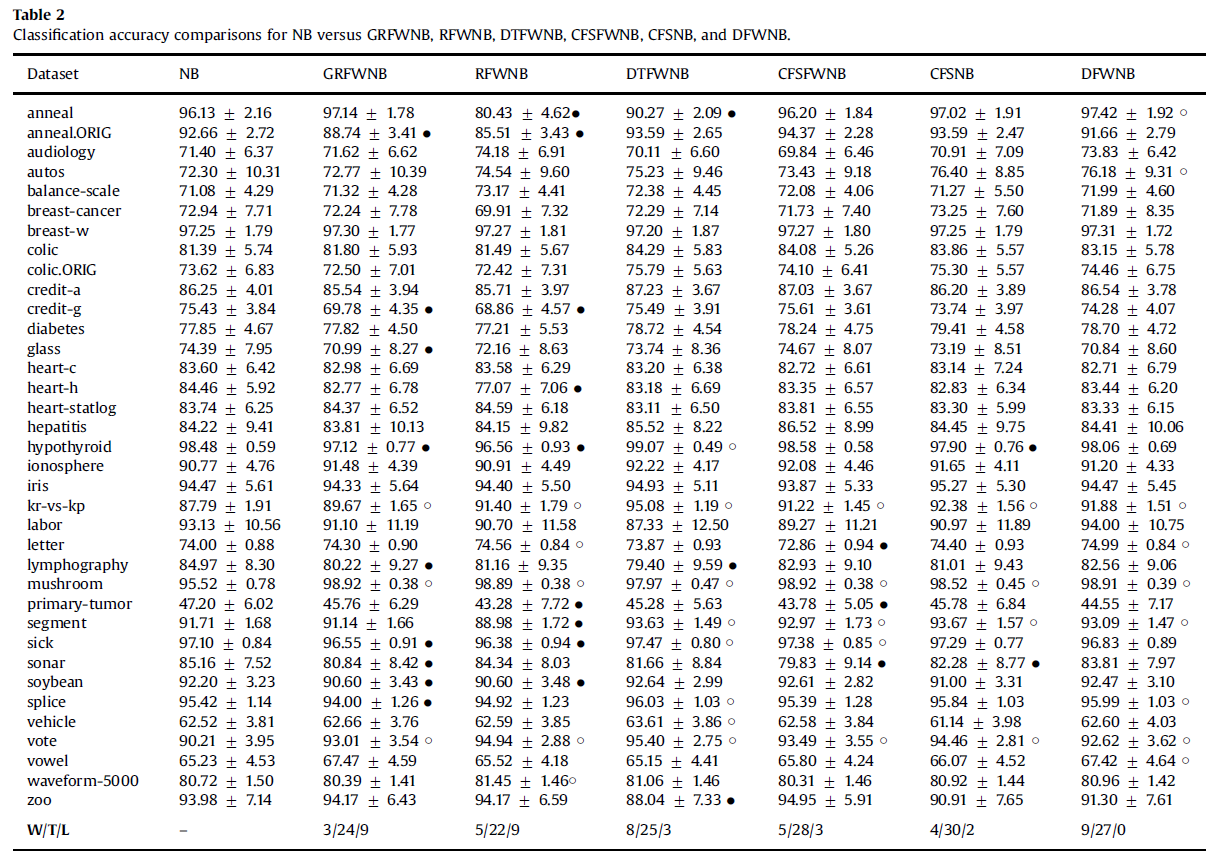
\includegraphics[width=\linewidth]{images/article1/table2.png}
    \caption{}
    \label{a1_table2}
\end{figure}
\begin{figure}
    \centering
    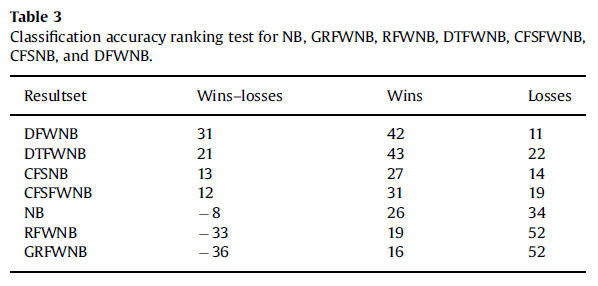
\includegraphics[width=\linewidth]{images/article1/table3.png}
    \caption{}
    \label{a1_table3}
\end{figure}

\clearpage

\begin{figure}
    \centering
    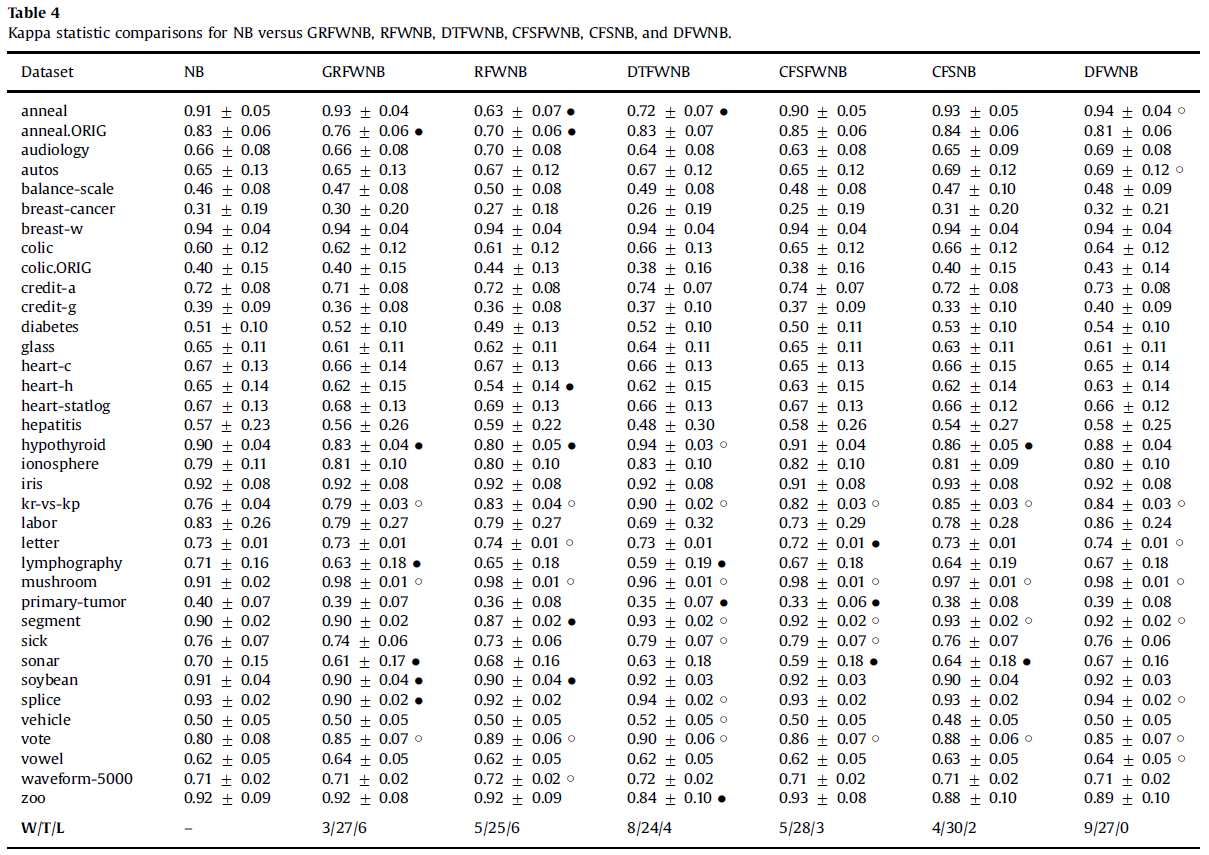
\includegraphics[width=\linewidth]{images/article1/table4.png}
    \caption{}
    \label{a1_table4}
\end{figure}
\begin{figure}
    \centering
    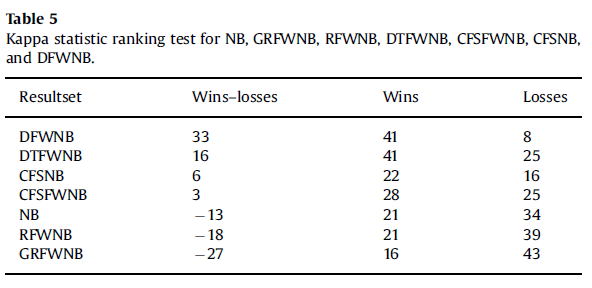
\includegraphics[width=\linewidth]{images/article1/table5.png}
    \caption{}
    \label{a1_table5}
\end{figure}

\clearpage

\begin{figure}
    \centering
    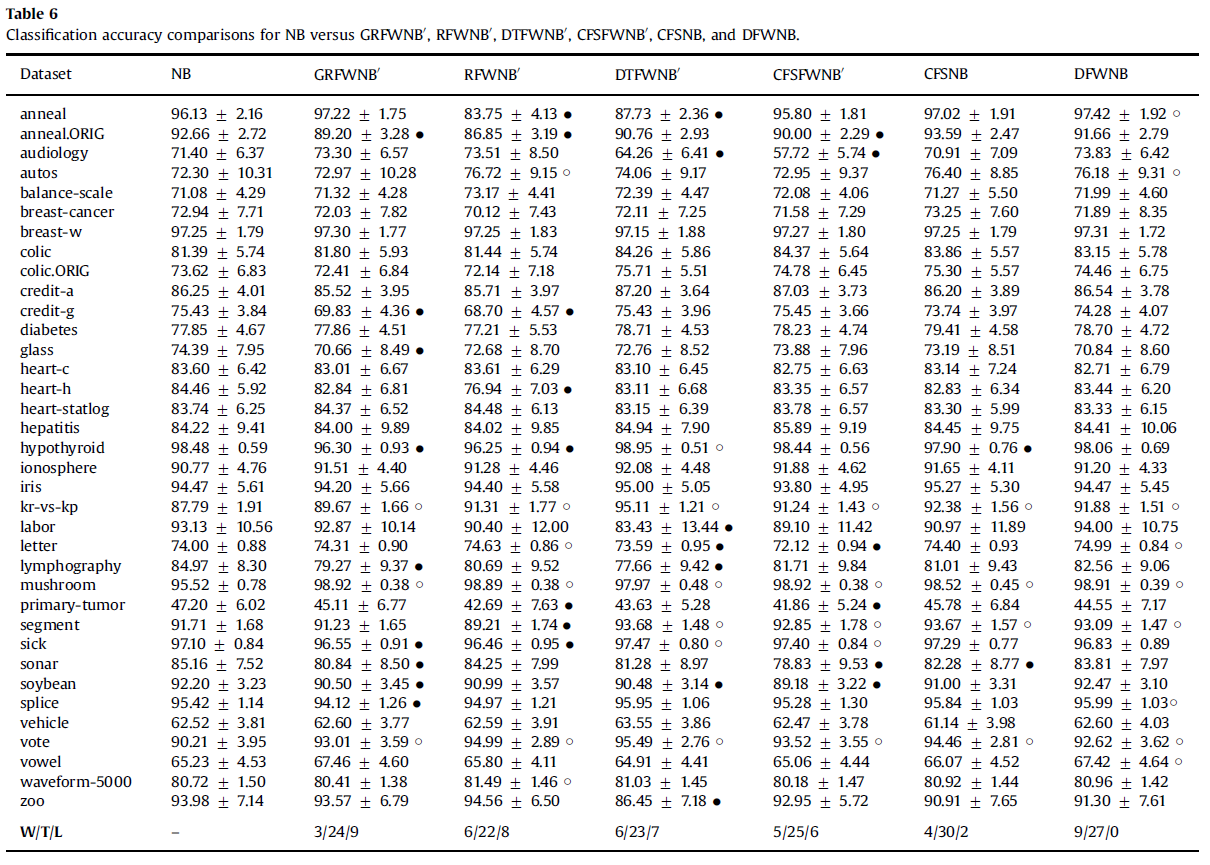
\includegraphics[width=\linewidth]{images/article1/table6.png}
    \caption{}
    \label{a1_table6}
\end{figure}
\begin{figure}
    \centering
    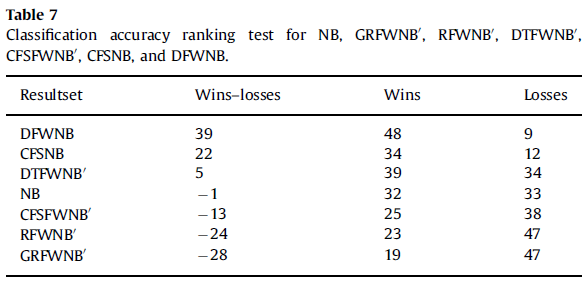
\includegraphics[width=\linewidth]{images/article1/table7.png}
    \caption{}
    \label{a1_table7}
\end{figure}

\clearpage

\begin{figure}
    \centering
    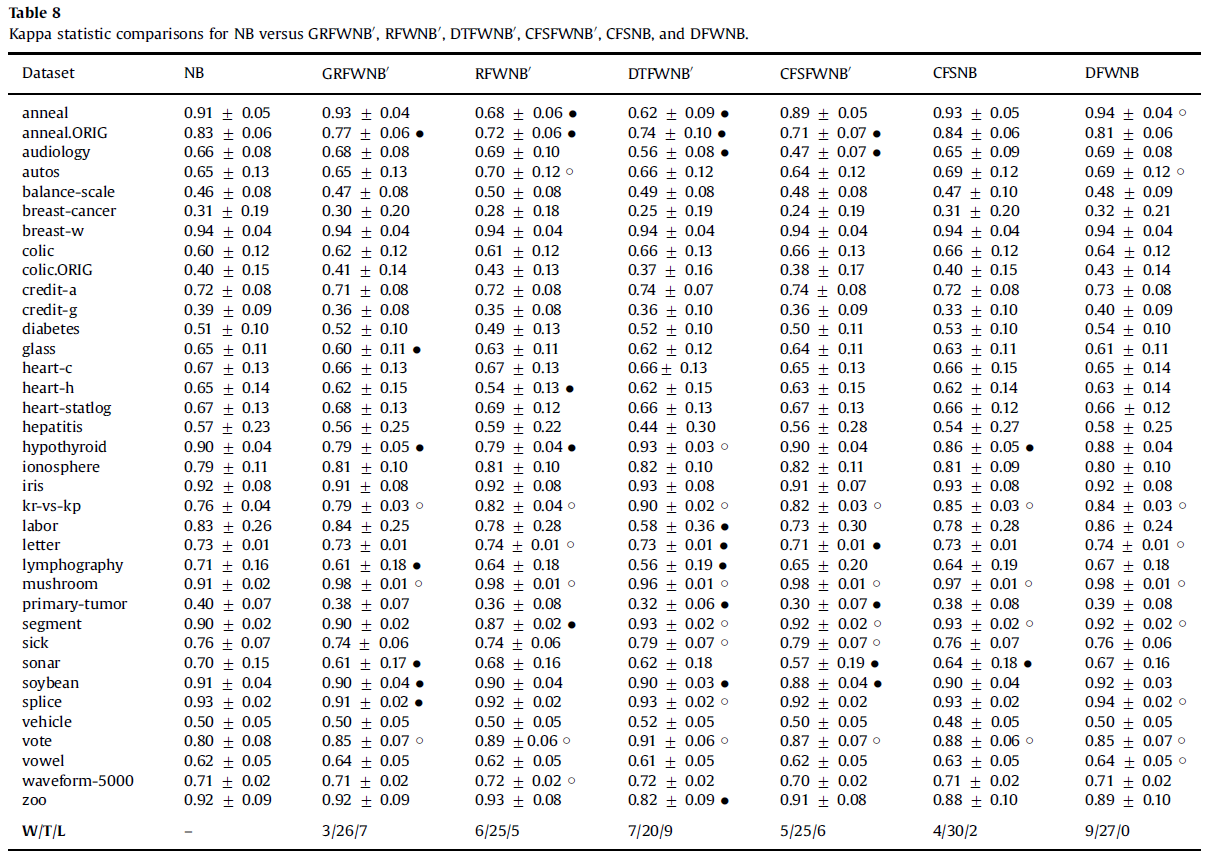
\includegraphics[width=\linewidth]{images/article1/table8.png}
    \caption{}
    \label{a1_table8}
\end{figure}
\begin{figure}
    \centering
    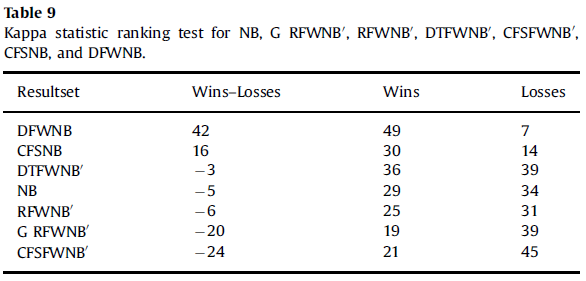
\includegraphics[width=\linewidth]{images/article1/table9.png}
    \caption{}
    \label{a1_table9}
\end{figure}

\clearpage

\begin{figure}
    \centering
    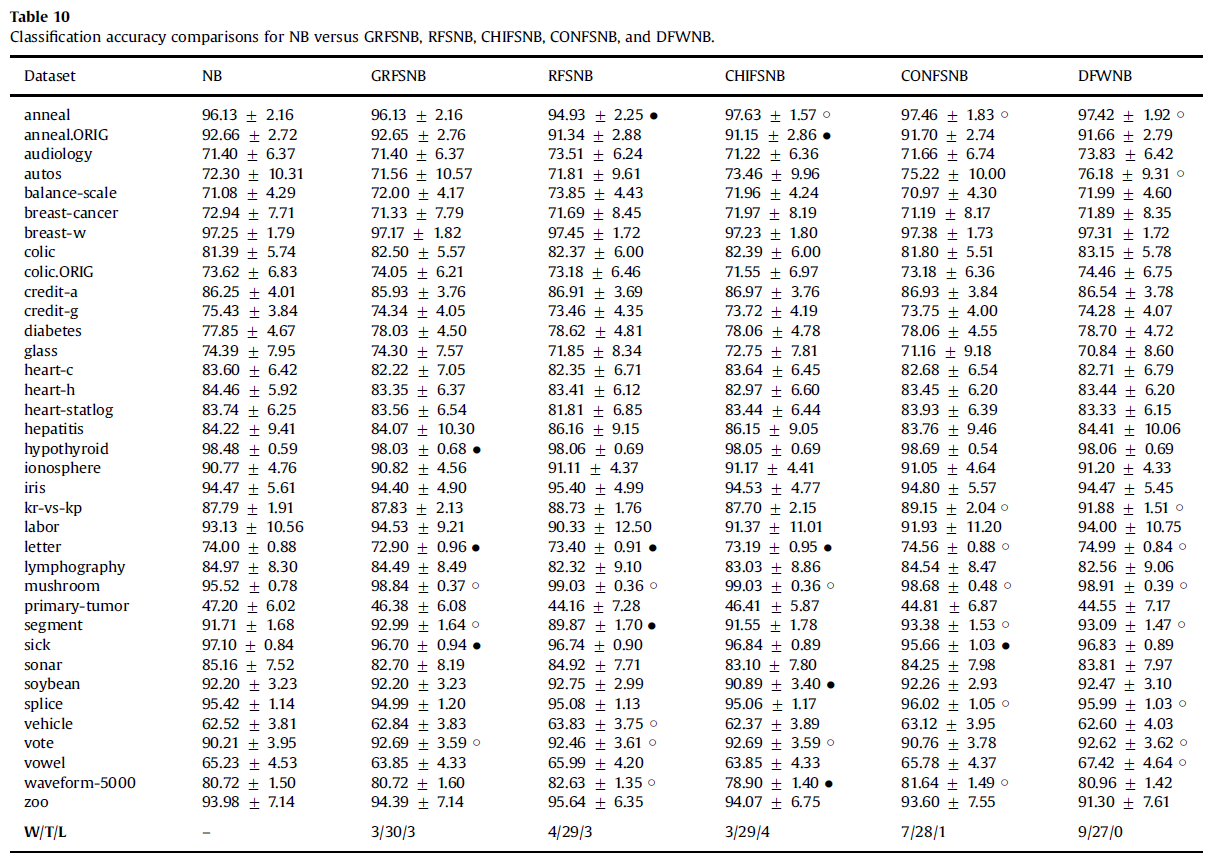
\includegraphics[width=\linewidth]{images/article1/table10.png}
    \caption{}
    \label{a1_table10}
\end{figure}
\begin{figure}
    \centering
    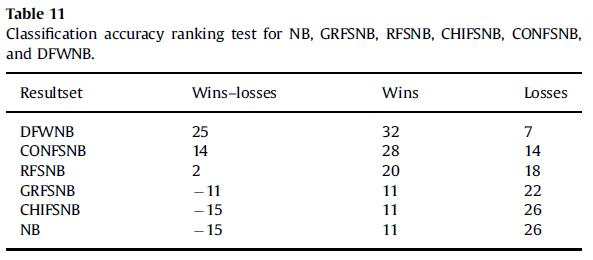
\includegraphics[width=\linewidth]{images/article1/table11.png}
    \caption{}
    \label{a1_table11}
\end{figure}

\clearpage

\begin{figure}
    \centering
    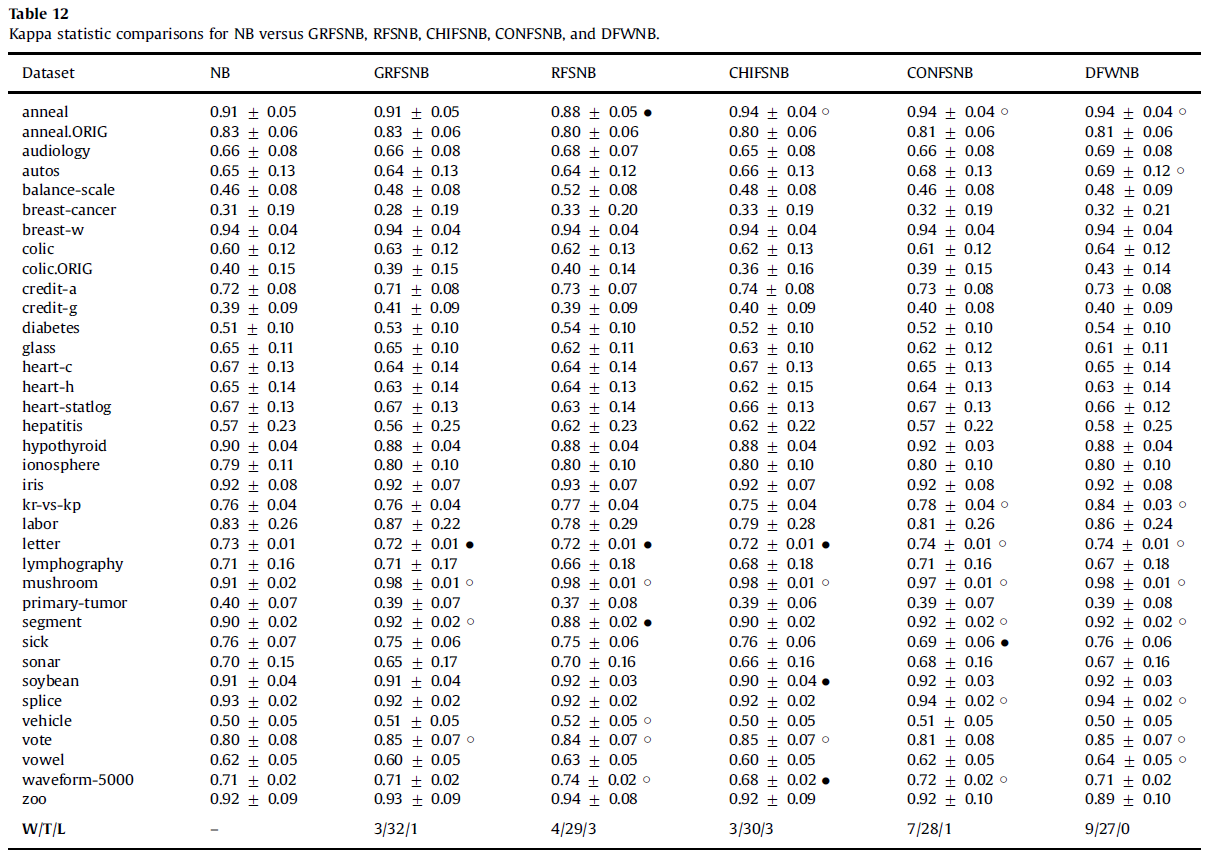
\includegraphics[width=\linewidth]{images/article1/table12.png}
    \caption{}
    \label{a1_table12}
\end{figure}
\begin{figure}
    \centering
    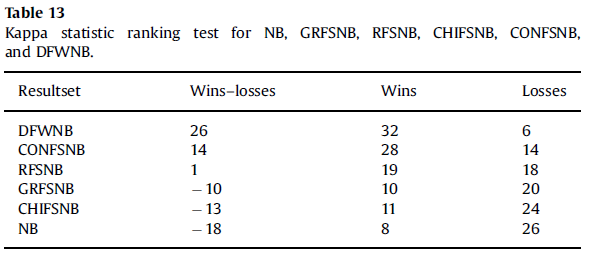
\includegraphics[width=\linewidth]{images/article1/table13.png}
    \caption{}
    \label{a1_table13}
\end{figure}

\clearpage

\begin{figure}
    \centering
    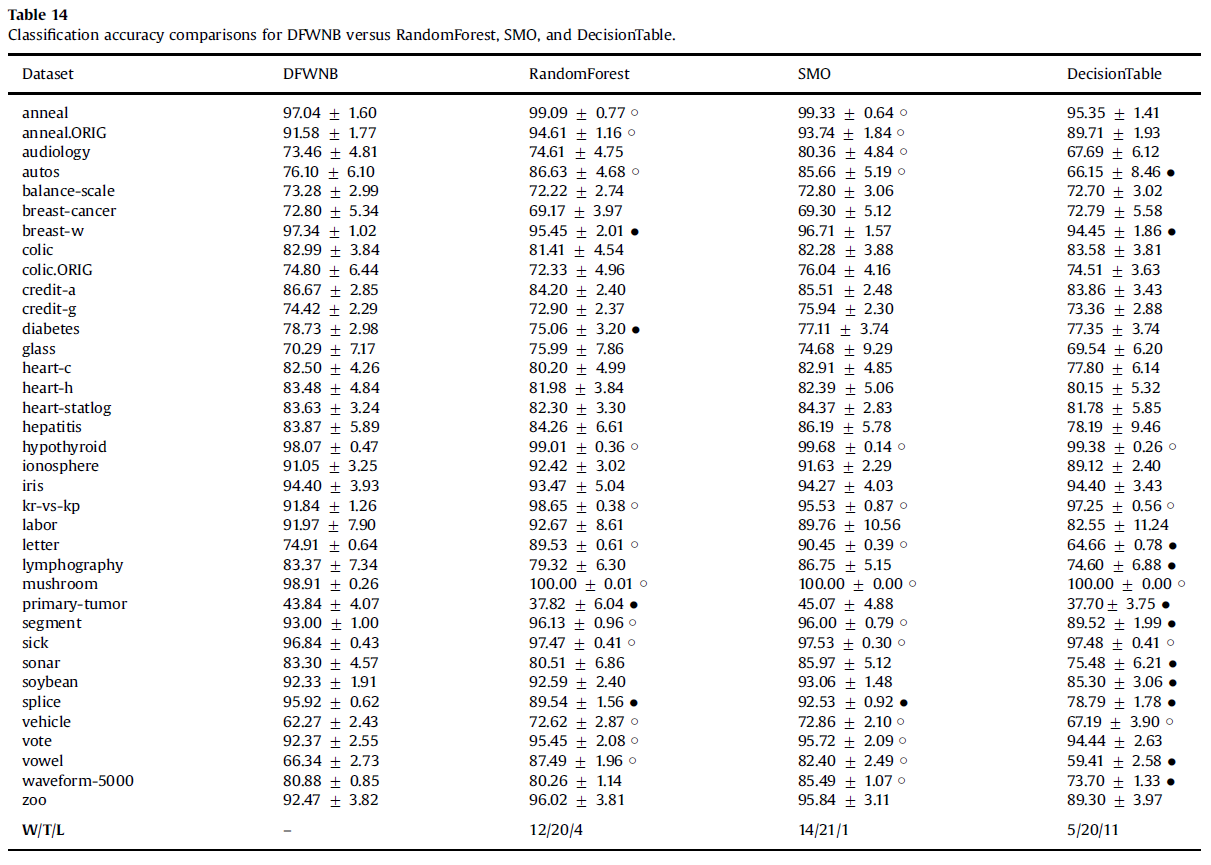
\includegraphics[width=\linewidth]{images/article1/table14.png}
    \caption{}
    \label{a1_table14}
\end{figure}
\begin{figure}
    \centering
    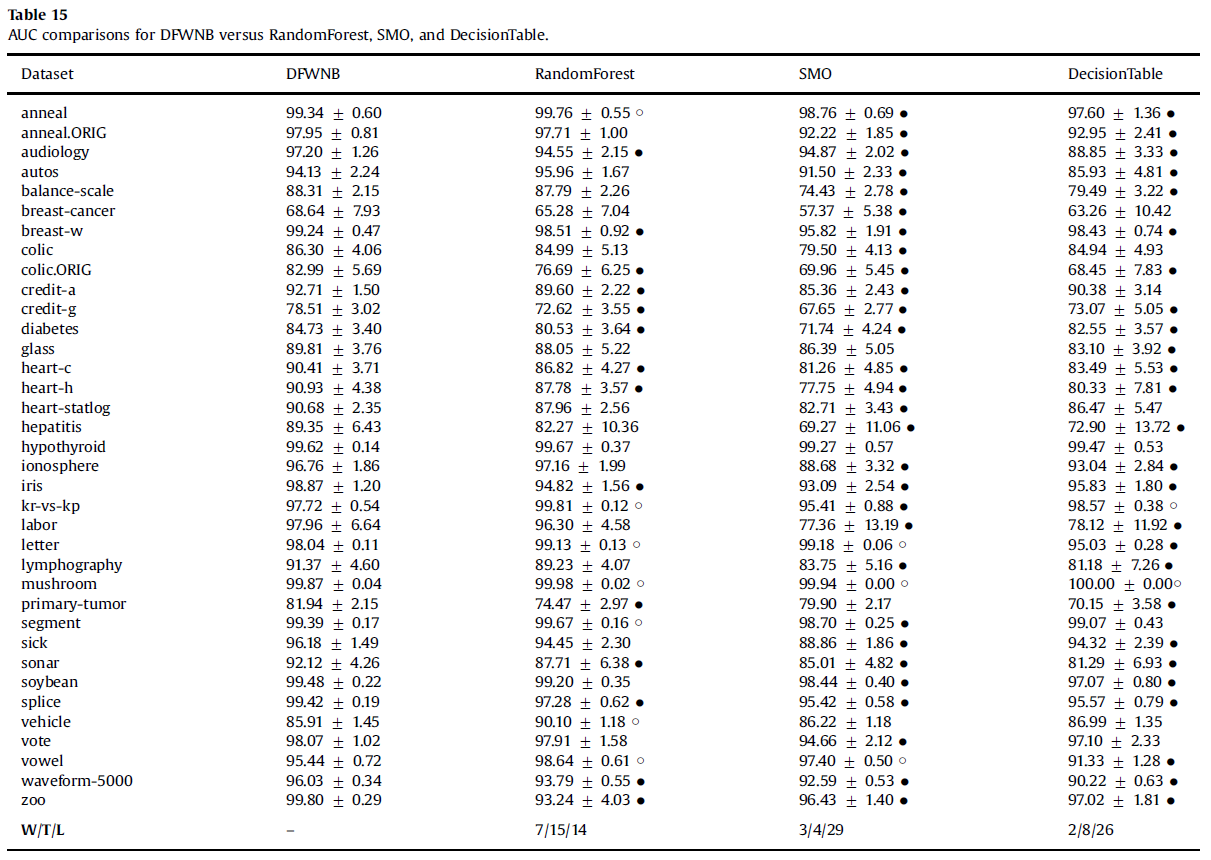
\includegraphics[width=\linewidth]{images/article1/table15.png}
    \caption{}
    \label{a1_table15}
\end{figure}

\clearpage

\begin{figure}
    \centering
    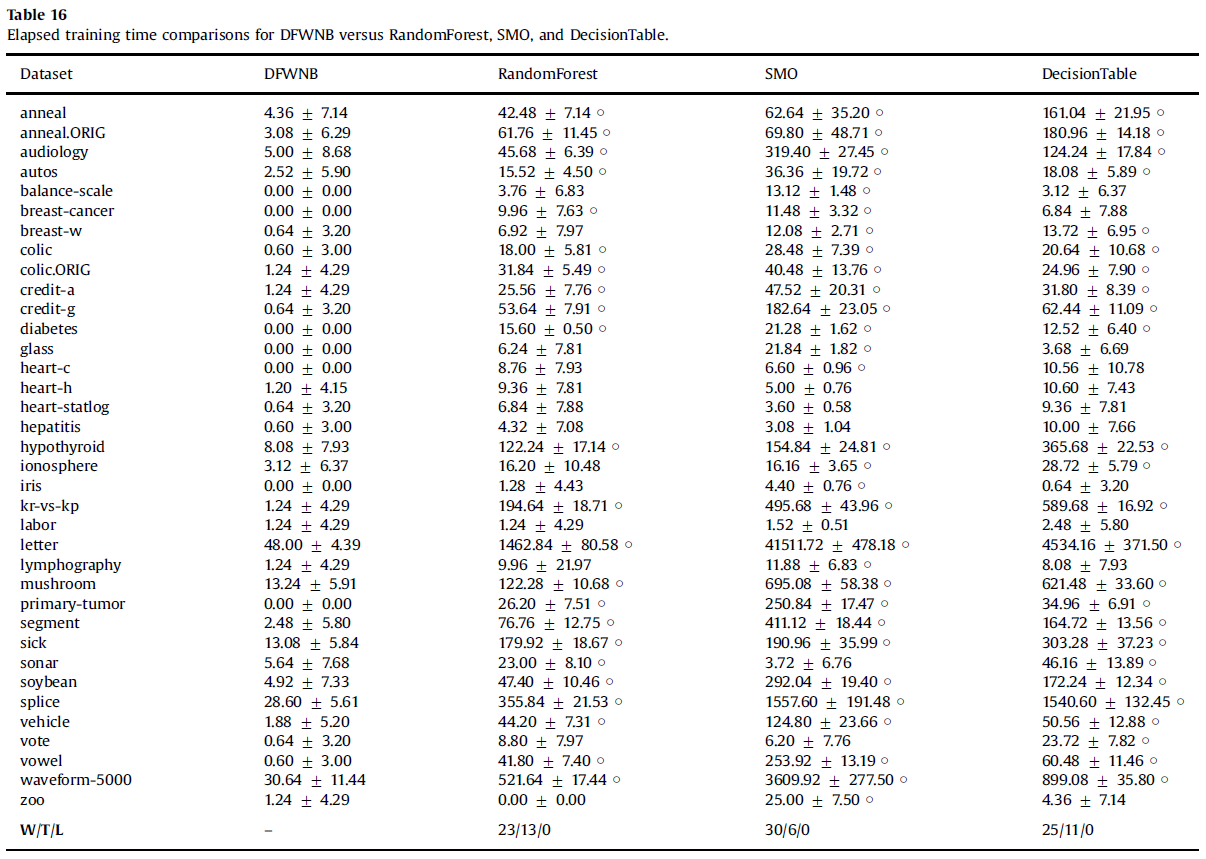
\includegraphics[width=\linewidth]{images/article1/table16.png}
    \caption{}
    \label{a1_table16}
\end{figure}
\begin{figure}
    \centering
    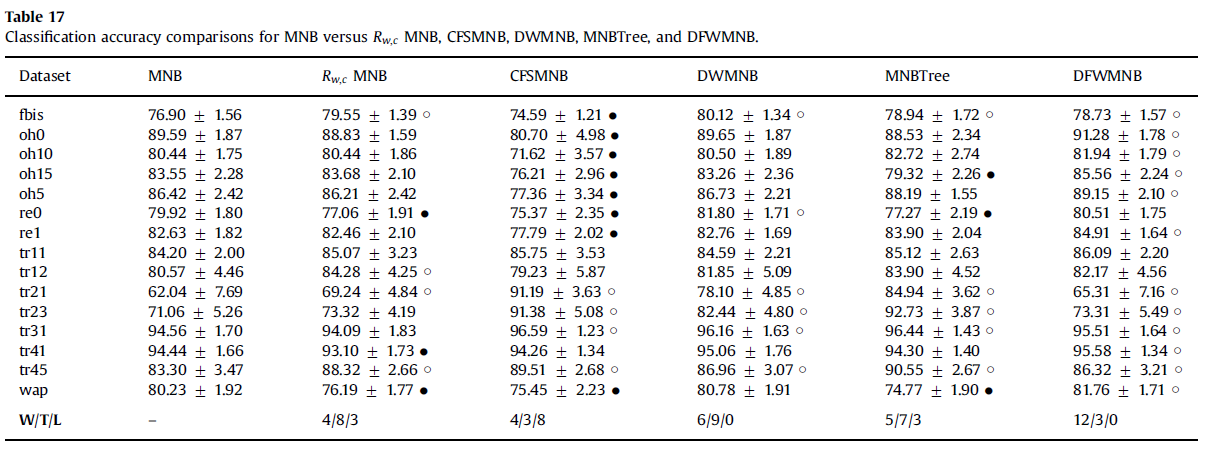
\includegraphics[width=\linewidth]{images/article1/table17.png}
    \caption{}
    \label{a1_table17}
\end{figure}

\clearpage

\begin{figure}
    \centering
    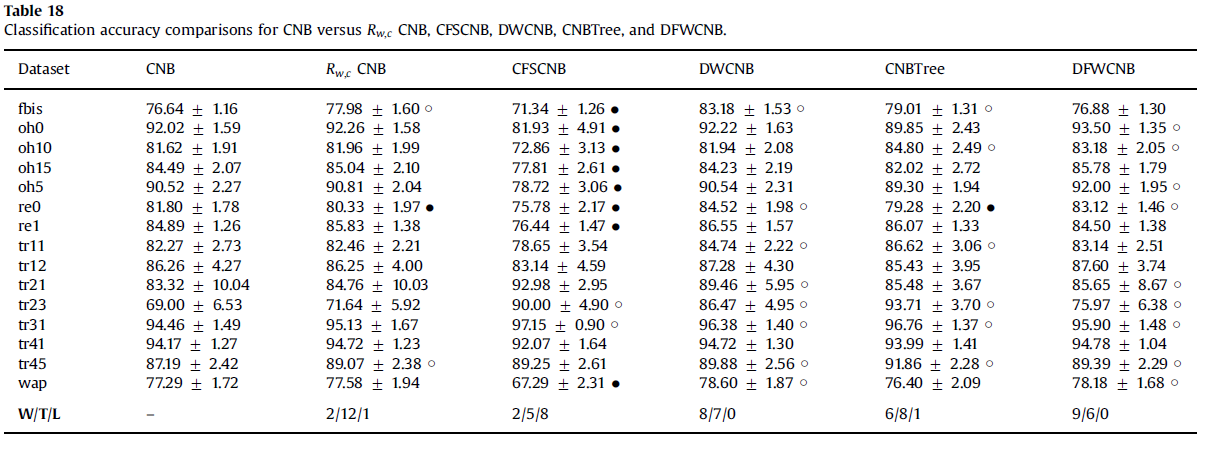
\includegraphics[width=\linewidth]{images/article1/table18.png}
    \caption{}
    \label{a1_table18}
\end{figure}

\begin{figure}
    \centering
    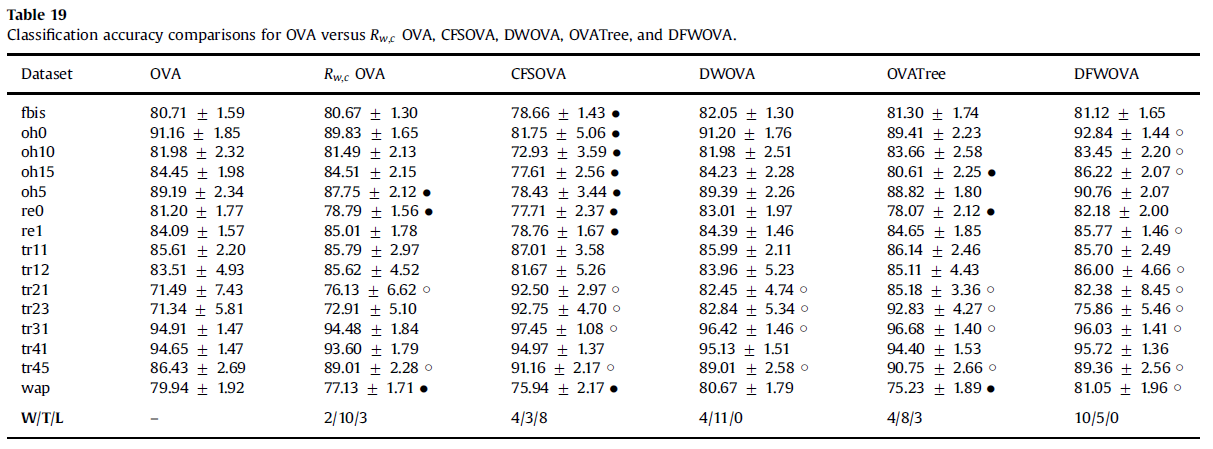
\includegraphics[width=\linewidth]{images/article1/table19.png}
    \caption{}
    \label{a1_table19}
\end{figure}

\clearpage

\section*{مقاله دوم}

در این مقاله مشابه مقاله اول پژوهشگران سعی دارند روش \lr{naive Bayes} را با وزن‌دهی
ویژگی‌ها بهبود دهند. رویکرد آن‌ها برای انجام این کار با مقاله اول اندکی متفاوت است.
در مقاله اول هم در تابع دسته‌بندی و هم در تابع احتمال شرطی تغییراتی انجام شده است،
اما در این مقاله، مشابه مقاله‌های پیش از مقاله اول، وزن ویژگی‌ها تنها در تابع دسته‌بندی اعمال می‌شود.
در جدول \ref{second_article} مشخصات کلی این مقاله آورده شده است.

\begin{table}[h]
    \centering
    \caption{مشخصات مقاله دوم}
    \label{second_article}
    \begin{tabular}{c|p{.7\linewidth}}
        مشخصه       & توضیح \\
        \hline
        عنوان مقاله & \lr{A Correlation-Based Feature Weighting Filter for Naive Bayes} \\
        سال انتشار  & 2018
    \end{tabular}
\end{table}

\subsection*{روش پیشنهادی}

در ادامه فرمول‌هایی که این مقاله برای دسته‌بندی \lr{naive Bayes} استفاده می‌کند، آورده شده است.
این فرمول‌ها در بیشتر مقالاتی که روش \lr{naive Bayes} را با استفاده از وزن‌دهی ویژگی‌ها بهبود می‌دهند،
دیده می‌شود. در این فرمول‌ها، برخلاف فرمول‌های ارائه شده در مقاله اول،
وزن ویژگی‌ها تنها در فرمول \ref{bayes_classification_formula}
اعمال شده و باقی فرمول‌ها نسبت به روش \lr{naive Bayes} بدون تغییر باقی مانده است.

\begin{eqnarray}
    P(c) & = & \frac{1}{n+1} (\sum_{i=0}^{n} \delta(c_i, c) + \frac{1}{k}) \\
    P(a_i|c) & = & \frac{\sum_{j=0}^{n} \delta(a_j, a_i) \delta(c_j, c) + \frac{1}{n}}{\sum_{j=1}^{n} \delta(c_j,c) + 1} \\
    c(x) & = & \argmax_{c \in C} P(c) \prod_{i=1}^{m} P(a_i|c)^{W_i} \label{bayes_classification_formula}
\end{eqnarray}

در فرمول‌های بالا منظور از $n$ تعداد دسته داده‌ها، منظور از $k$ تعداد مقادیر ممکن برای دسته $c$ و
منظور از $W_i$ وزن متناظر ویژگی $a_i$ بوده و تابع $\delta$ به صورت زیر تعریف می‌شود.

\begin{eqnarray}
    \delta(x, y) =
    \begin{cases}
        1 & x = y \\
        0 & x \neq y
    \end{cases}
\end{eqnarray}

در فرمول‌های بالا چالش اصلی تعیین مقدار $W_i$ برای
ویژگی‌های مختلف است. در این مقاله با ارائه روشی به نام \lr{Correlation-based Feature Weighting} که به اختصار
\lr{CFW} نامیده می‌شود، روشی برای تعیین مقدار $W_i$ها پیشنهاد می‌شود.

شهود پشت روش ارائه شده توسط این مقاله مشابه شهود روش \lr{CFS} است:
ویژگی‌هایی که با برچسب دسته همبستگی بالایی دارند ولی با دیگر ویژگی‌‌ها همبستگی پایینی دارند، سهم بزرگی در دسته‌بندی داشته و در نتیجه
باید $W_i$ بزرگی داشته باشند.

در این روش برخلاف روش \lr{CFS} یک گروه از ویژگی‌ها انتخاب و به عنوان گروه ویژگی‌های بهینه ارائه نمی‌شوند، بلکه به
هر یک از ویژگی‌ها وزنی بین صفر و یک نسبت داده می‌شود. بعلاوه در این روش به جای محاسبه معیار همبستگی از
معیار \lr{Mutual Information} استفاده می‌شود. روش \lr{CFW} برخلاف روش \lr{CFS} تنها برای کمیت‌های
کیفی قابل اعمال بوده و برای کمیت‌های کمی کاربرد ندارد.

برای محاسبه \lr{CFW} در ابتدا نیاز است \lr{mutual information} بین دو ویژگی و بین ویژگی و برچسب هر دسته
به صورت زیر محاسبه شود. در فرمول‌های زیر منظور از $C$ برچسب هر دسته،
منظور از $A_i$ و $A_j$ دو ویژگی مختلف از مجموعه ویژگی‌های
داده‌ها و متغیر‌های $c$، $a_i$ و $a_j$ به ترتیب نشان دهنده مقادیری است که به هر یک از متغیر‌های $C$،
$A_i$ و $A_j$ نسبت داده می‌شود.

\begin{eqnarray}
    I(A_i; C) & = & \sum_{a_i}\sum_{c} P(a_i, c) \log\frac{P(a_i, c)}{P(a_i)P(c)} \\
    I(A_i; A_j) & = & \sum_{a_i}\sum_{a_j} P(a_i, a_j) \log \frac{P(a_i, a_j)}{P(a_i) P(a_j)}
\end{eqnarray}

پس از محاسبه مقادیر بالا به ازای ویژگی‌های مختلف، مقادیر حاصل شده با تقسیم بر میانگین نرمال می‌شوند.
به عبارت ریاضی

\begin{eqnarray}
    NI(A_i; C) & = & \frac{I(A_i; C)}{\frac{1}{m}\sum_{i=1}^{m}I(A_i; C)} \\
    NI(A_i; A_j) & = & \frac{I(A_i; A_j)}{\frac{1}{m(m-1)}\sum_{i=1}^{m}\sum_{j=1 \wedge  j\neq i}^{m} I(A_i; A_j)}
\end{eqnarray}

در ادامه با استفاده از این مقادیر نرمال حاصل شده، متغیر $D_i$ محاسبه می‌شود. دقت شود که تا قبل از محاسبه
$D_i$ هنوز در واقعیت هیچ حرکتی برای محاسبه وزن‌ها صورت نگرفته است و تنها پیش نیاز‌های اولیه لازم محاسبه شده است.
اما در $D_i$ شهودی که از الگوریتم در نظر داریم، اعمال می‌شود. به نوعی محاسبه $D_i$ اولین گام موثر الگوریتم است.

\begin{eqnarray}
    D_i = NI(A_i; C) - \frac{1}{m-1} \sum_{j=1 \wedge j\neq i}^{m} NI(A_i; A_j)
\end{eqnarray}

از آن جا که مقدار $D_i$ بین صفر و یک نیست و حتی ممکن است برای بعضی از ویژگی‌ها منفی شود، بنابراین این معیار
به تنهایی نمی‌تواند به عنوان وزن الگوریتم \lr{naive Bayes} استفاده شود. اما می‌توان با استفاده از تابعی ساده
مانند سیگموید، می‌توان مقدار $D_i$ را به بازه صفر و یک نگاشت کرد. به عبارت دقیق‌تر در این مقاله وزن‌های مورد استفاده
به صورت زیر با استفاده از تابع سیگموید به دست می‌آید.

\begin{eqnarray}
    W_i = \frac{1}{1+e^{-D_i}}
\end{eqnarray}

\subsection*{استفاده از روش \lr{CFW} در داده‌های متنی}

در این مقاله روش وزن‌دهی پیشنهادی بر روی دو روش پایه \lr{MNB} و \lr{CNB}
اعمال شده است. در این مقاله، بر خلاف مقاله اول، روش وزن‌دهی بر روی \lr{OVA}
اعمال نشده است. شیوه اعمال وزن‌دهی برای هر یک از روش‌های \lr{MNB} و \lr{CNB}
در ادامه بیان می‌شود.

اعمال روش وزن‌دهی بر روی \lr{MNB}.

\begin{eqnarray}
    P(c) & = & \frac{\sum_{j=1}^{n}\delta(c_j, c) + 1/k}{n+1} \\
    P(w_i|c) & = & \frac{\sum_{j=1}^{n} f_{ji}\delta(c_j, c) + 1/m}{\sum_{i=1}^{m}\sum_{j=1}^{n}f_{ji}\delta(c_j,c)+1} \\
    c(d) & = & \argmax_{c \in C} \Bigl(\log P(c) + \sum_{i=1}^{m} W_i f_i \log P(w_i| c)\Bigr)
\end{eqnarray}

اعمال روش وزن‌دهی بر روی \lr{CNB}.

\begin{eqnarray}
    P(\bar{c}) & = & \frac{\sum_{j=1}^{n}\delta(c_j, \bar{c}) + 1/k}{n+1} \\
    P(w_i|\bar{c}) & = & \frac{\sum_{j=1}^{n} f_{ji}\delta(c_j, \bar{c}) + 1/m}{\sum_{i=1}^{m}\sum_{j=1}^{n}f_{ji}\delta(c_j,\bar{c})+1} \\
    c(d) & = & \argmin_{c \in C} \Bigl(\log P(\bar{c}) + \sum_{i=1}^{m} W_i f_i \log P(w_i| \bar{c})\Bigr)
\end{eqnarray}

اگر به خاطر داشته باشید، روش \lr{CFW} تنها برای داده‌های کیفی کارایی داشت، اما در این‌جا
با تعداد کلمه‌ها در متن سروکار داریم. برای رفع این مشکل باید تعداد تکرار کلمه
به مقادیر کیفی تبدیل شود. برای این کار دو دسته در نظر گرفته می‌شود. دسته اول کلمات با
تکرار غیرصفر و دسته دوم کلمات با تکرار صفر. به زبان ریاضی \lr{mutual information}
بین دو کلمه و یا کلمه و دسته را به شکل زیر محاسبه می‌کنیم. باقی مراحل همانند روال
عادی طی می‌شود.

\begin{eqnarray}
    I(w_i; C) & = & \sum_{f_i \in \{0, \bar{0}\}}\sum_{c} P(f_i, c) \log\frac{P(f_i, c)}{P(f_i)P(c)} \\
    I(w_i; w_j) & = & \sum_{f_i \in \{0, \bar{0}\}}\sum_{a_j} P(f_i, f_j) \log \frac{P(f_i, f_j)}{P(f_i) P(f_j)}
\end{eqnarray}

\subsection*{نتایج}

نتایج روش ارائه شده در این مقاله در شکل‌های موجود در صفحات آینده آورده می‌شود.
با توجه به آن که در این مقاله یک روش وزن‌دهی عام‌منظوره برای بهبود مدل
\lr{naive Bayes} ارائه شده و سپس این روش به طور خاص روی داده‌های متنی آزمایش
شده است، بنابراین می‌توان نتایج را به دو گروه تقسیم کرد. در گروه اول از ۳۶
مجموعه داده دانشگاه \lr{UCI} و در گروه دوم از ۱۵ مجموعه داده
متنی که در دسترس عموم قرار دارد، برای نشان دادن کارا بودن روش استفاده شده است.
در ادامه ابتدا نتایج حاصل از گروه اول مورد بررسی قرار می‌گیرد و سپس
نتایج مربوط به گروه دوم.

روش‌های مختلف مورد بحث در محیط \lr{Weka} پیاده‌سازی شده است. برای گزارش نتایج،
الگوریتم مد نظر ۱۰ مرتبه روی مجموعه دادگان اجرا می‌شود. در هر مرتبه
اجرا الگوریتم داده‌های آموزشی و تست با استفاده از روش
\lr{10-Fold cross validation} تعیین می‌شود.

روش‌های زیر برای بررسی عملکرد روش فعلی انتخاب شده‌اند.

\begin{itemize}
    \item \lr{NB}: روش بیز ساده بدون هیچ‌گونه بهبودی
    \item \lr{KLMFW}: روش وزن‌دهی مبتنی بر اندازه‌گیری \lr{Kullback-Leibler}
    \item \lr{GRFW}: روش وزن‌دهی مبتنی بر \lr{gain ratio}
    \item \lr{DTFW}: روش وزن‌دهی با استفاده از درخت‌های تصمیم
    \item \lr{DFW}: روش وزن‌دهی عمیق. این روش همان روش ارائه شده در مقاله اول است.
    \item \lr{DEFW}: روش وزن‌دهی مبتنی بر بهبود تفاوت
    \item \lr{CLLFW}: روش وزن‌دهی مبتنی بر \lr{conditional log likelihood}
    \item \lr{MSEFW}: روش وزن‌دهی مبتنی بر \lr{mean squared error}
\end{itemize}

مجموعه دادگان استفاده شده برای مقایسه روش‌ها در حالت کلی در شکل \ref{a2_table4} آورده
شده است. بعضی از این مجموعه دادگان دارای \lr{missing value} هستند. استراتژی
استفاده شده برای حذف این مقادیر نامعلوم، پرکردن آن‌ها با میانگین مقادیر معلوم
برای داده‌های کمی و برای داده‌های کیفی پرکردن آن‌ها با مد داده‌های معلوم است.
عملکرد روش‌ها بر روی این داده‌ها در چهار حالت مختلف بررسی شده است که در ادامه
به صورت مختصر بررسی می‌شوند.

\begin{itemize}
    \item معیار صحت اولین معیاری است که برای بررسی عملکرد روش‌ها در نظر گرفته شده است.
          نتایج این روش در شکل \ref{a2_table5} مشاهده می‌شود.
          همان‌طور که مشاهده می‌شود، عملکرد روش \lr{CFW} از بسیاری از روش‌های دیگر بهتر است.
          اما این به این معنی نیست که این روش بهترین عملکرد را داشته است. الگوریتم‌های
          \lr{CLLFW} و \lr{MSEFW} نسبت به این روش به نتایج بهتری دست پیدا کرده‌اند.
          با توجه به این که هر دو این روش‌ها جزو روش‌های \lr{wrapper} بوده و نه
          \lr{filter} بنابراین می‌توان بهتر بودن عملکرد آن‌ها را منطقی دانست.
          جدول عملکرد روش‌ها بر حسب صحت نتایج از جنبه‌های دیگر مانند روش \lr{t-test} و
          \lr{wilcoxon-text} نیز مورد بررسی قرار گرفته است که نتایج آن‌ها به ترتیب
          در همان شکل \ref{a2_table5} و \ref{a2_table6} مشاهده می‌شود.
    \item الگوریتم‌ها با استفاده از معیار \lr{Conditional Log Likelihood}
          نیز بررسی شده‌اند. با نگاه کردن به نتایج که در شکل‌ \ref{a2_table7}
          آورده شده است، نیز شاهد عملکرد مناسب الگوریتم هستیم. در شکل
          \ref{a2_table8} نیز بررسی نتایج حاصل از این الگوریتم با استفاده از تست
          \lr{wilcoxon} مشاهده می‌شود.
    \item جنبه دیگری که برای بررسی عملکرد مدل‌ها استفاده شده است، سطح زیر نمودار
          یا \lr{AUC} است. نتایج این روش در جدول \ref{a2_table9} آورده شده است.
          در این جدول نیز عملکرد ممتاز روش ارائه شده در این مقاله نسبت به روش‌های
          مبتنی بر فیلتر را شاهد هستیم. اما در این جنبه نیز عملکرد روش \lr{CLLFW} و
          \lr{MSEFW} نسبت به روش مقاله عملکرد بهتری دارد. نتایج موجود در شکل \ref{a2_table9}
          همانند نتایج قبلی با استفاده از دو تست \lr{wilcoxon} و \lr{t-test} نیز
          بررسی شده‌اند.
    \item در نهایت روش‌های مختلف از جنبه زمان مورد نیاز برای آموزش بررسی شده‌اند.
          از این لحاظ عملکرد متوسطی را از الگوریتم شاهد هستیم، چرا که تقریبا از نصف روش‌ها
          به زمان کم‌تر و از نصف دیگر به زمان بیشتری نیاز دارد.
\end{itemize}

برای بررسی عملکرد الگوریتم در داده‌های متنی از مجموعه دادگان موجود در شکل
\ref{a2_table13}، استفاده شده است. این مجموعه دادگان، به صورت آزاد در دسترس
همه قرار داشته و توسط مقالات مختلف برای بررسی عملکرد الگوریتم استفاده شده است.
نتایج حاصل از عملکرد مدل در شکل \ref{a2_figure} مشاهده می‌شود. در این حالت
مشخص است که با اعمال الگوریتم وزن دهی پیشنهاد شده بر روی روش‌های
\lr{MNB} و \lr{CNB} موجب بهبود عملکرد این روش‌ها شده است. نکته منفی که در نحوه ارائه نتایج این قسمت
به نظر می‌رسد، مقایسه روش وزن‌دهی پیشنهاد شده تنها با حالت عادی روش‌های \lr{MNB}
و \lr{CNB} است. در صورتی که در همین مقاله (و در مقاله اول مورد بررسی) روش‌های
مختلفی برای وزن‌دهی روش‌های \lr{naive Bayes} پیشنهاد شده است که ممکن بود با تست کردن
آن‌ها شاهد باشیم که عملکرد آن‌ها در این مجموعه دادگان بهتر از روش پیشنهادی است.
با مقایسه نتایج حاصل از این روش با روش پیشنهاد شده در مقاله اول، به این نتیجه می‌رسیم که
عملکرد هر دو الگوریتم در حالت استفاده از \lr{CNB} یکسان است اما الگوریتم پیشنهادی در
مقاله اول نسبت به \lr{CFW} عملکرد بهتری در حالت \lr{MNB} دارد.

\clearpage

\begin{figure}[h]
    \centering
    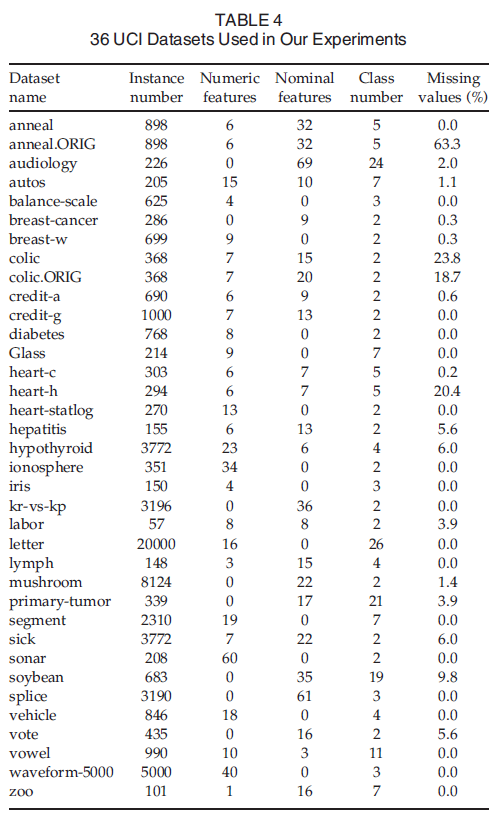
\includegraphics[width=\linewidth]{images/article2/table4.png}
    \caption{}
    \label{a2_table4}
\end{figure}

\clearpage

\begin{figure}
    \centering
    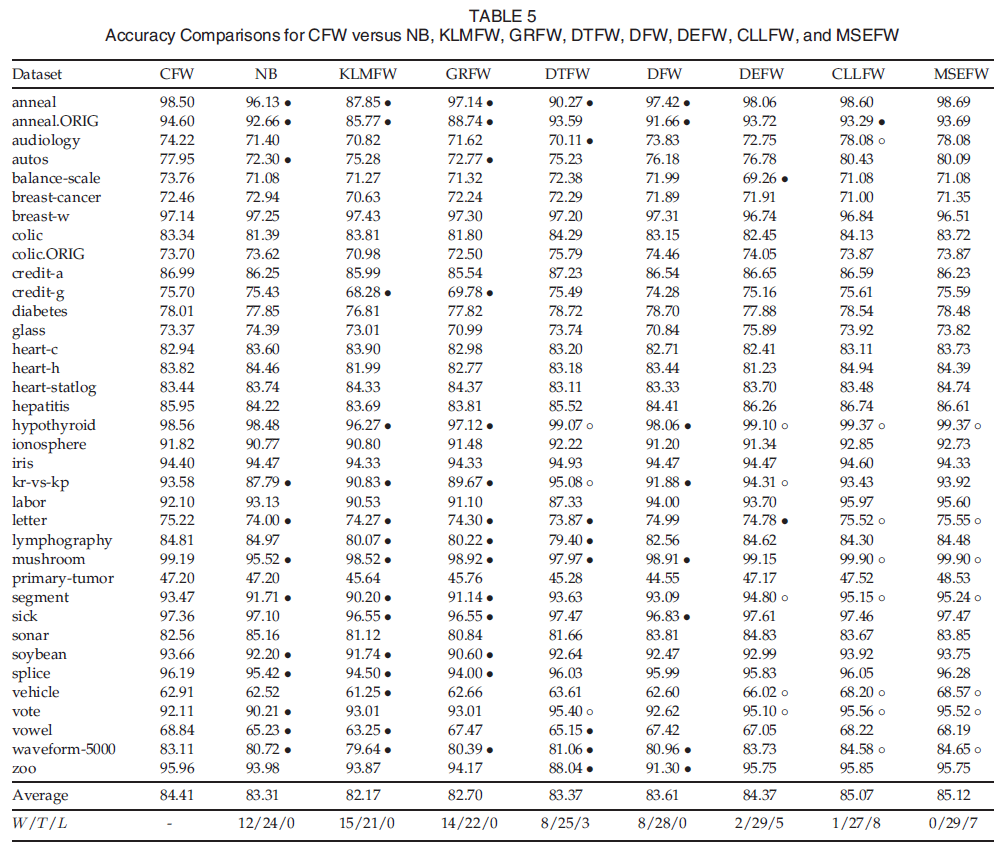
\includegraphics[width=\linewidth]{images/article2/table5.png}
    \caption{}
    \label{a2_table5}
\end{figure}

\begin{figure}
    \centering
    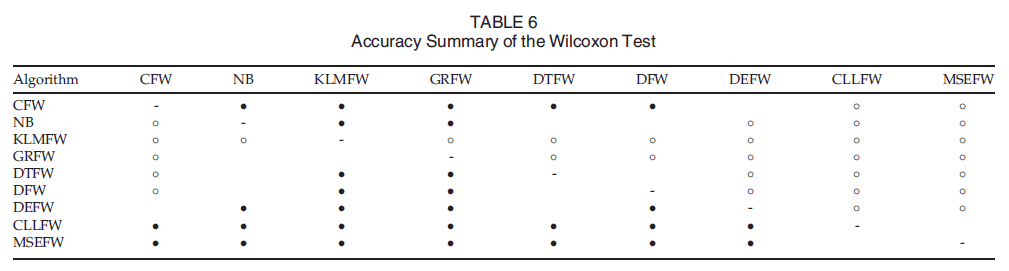
\includegraphics[width=\linewidth]{images/article2/table6.png}
    \caption{}
    \label{a2_table6}
\end{figure}

\clearpage

\begin{figure}
    \centering
    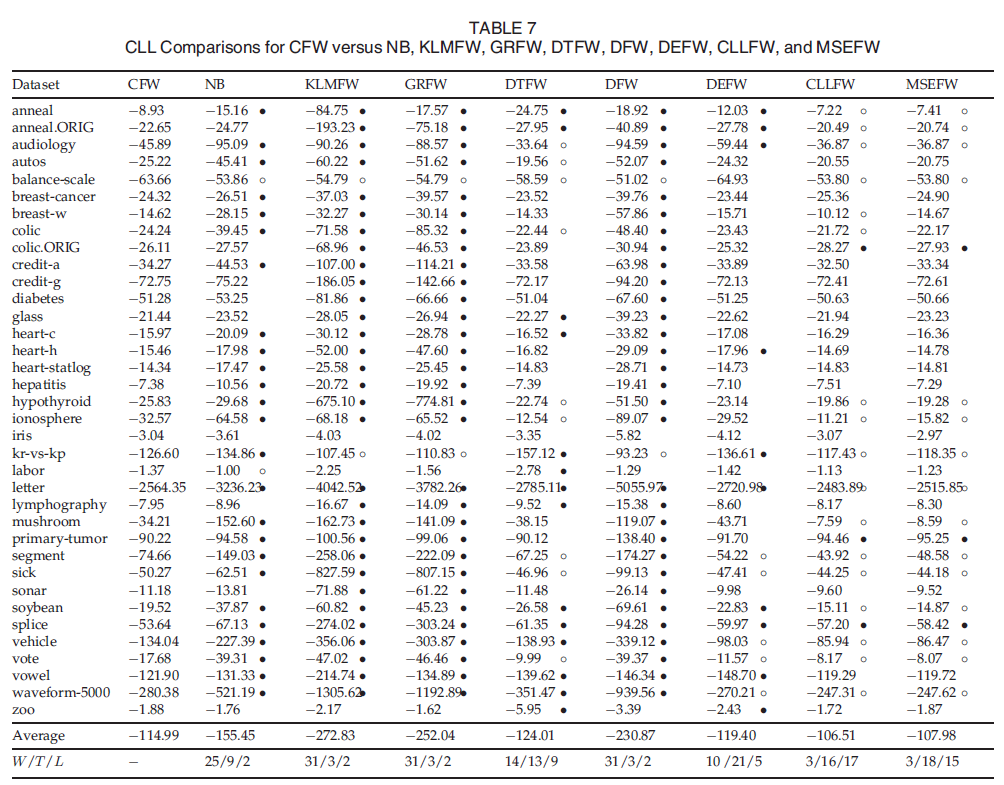
\includegraphics[width=\linewidth]{images/article2/table7.png}
    \caption{}
    \label{a2_table7}
\end{figure}

\begin{figure}
    \centering
    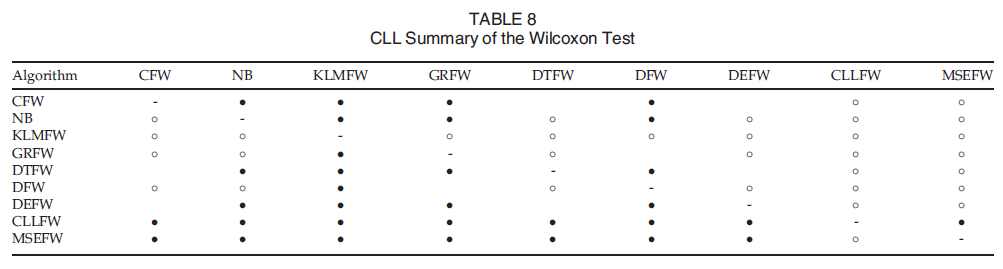
\includegraphics[width=\linewidth]{images/article2/table8.png}
    \caption{}
    \label{a2_table8}
\end{figure}

\clearpage

\begin{figure}
    \centering
    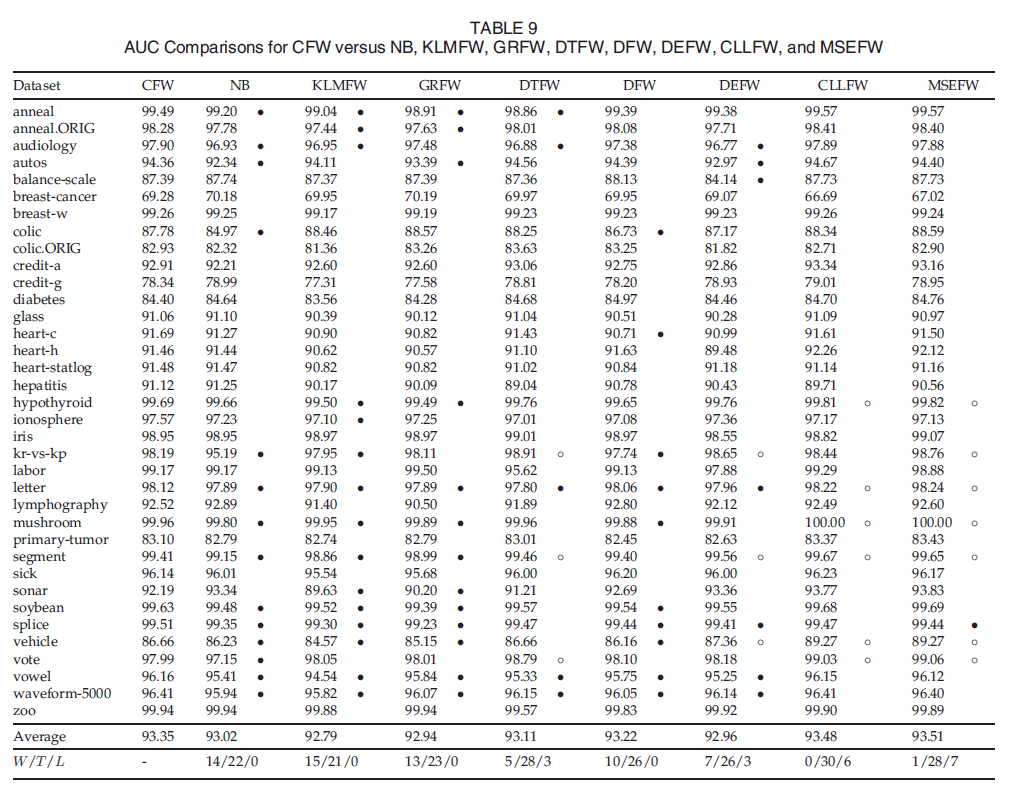
\includegraphics[width=\linewidth]{images/article2/table9.png}
    \caption{}
    \label{a2_table9}
\end{figure}

\begin{figure}
    \centering
    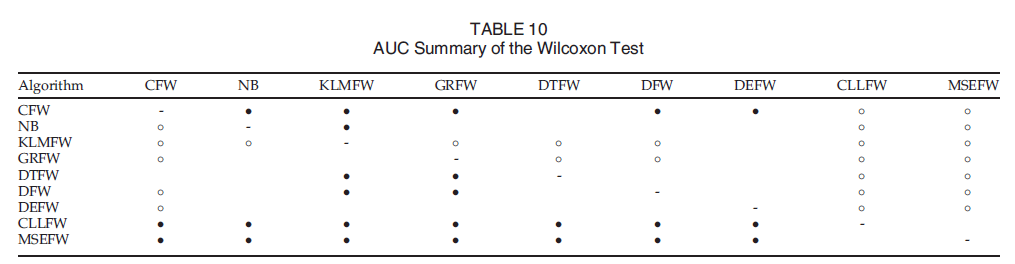
\includegraphics[width=\linewidth]{images/article2/table10.png}
    \caption{}
    \label{a2_table10}
\end{figure}

\clearpage

\begin{figure}
    \centering
    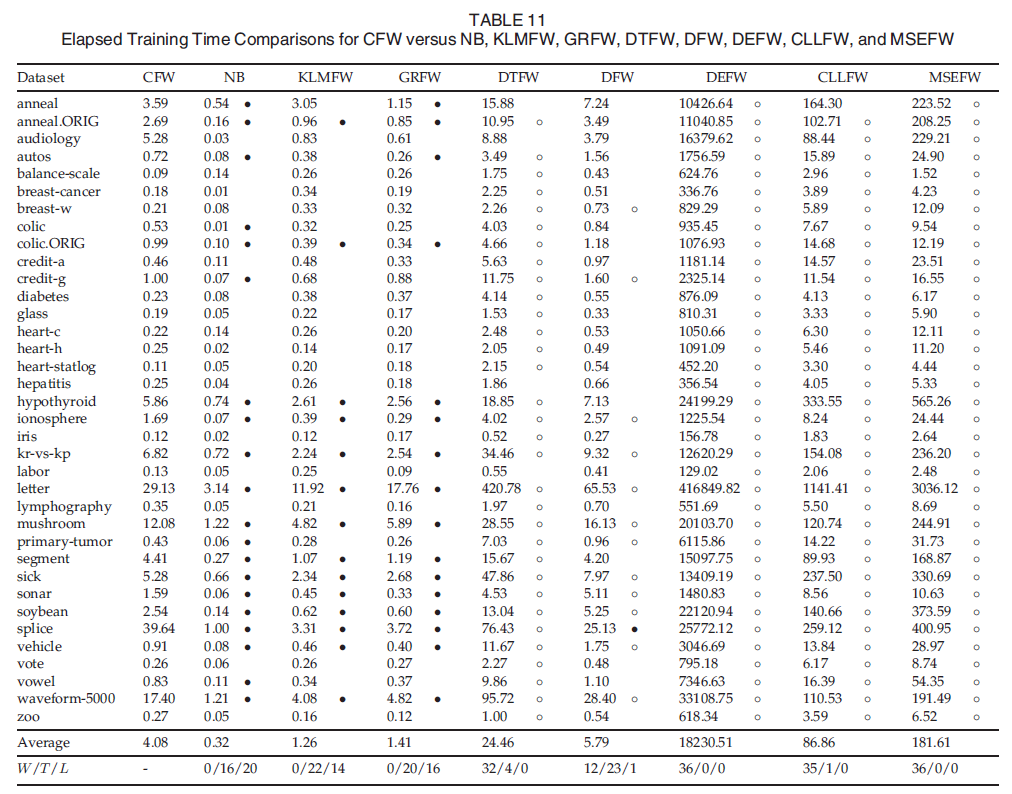
\includegraphics[width=\linewidth]{images/article2/table11.png}
    \caption{}
    \label{a2_table11}
\end{figure}

\begin{figure}
    \centering
    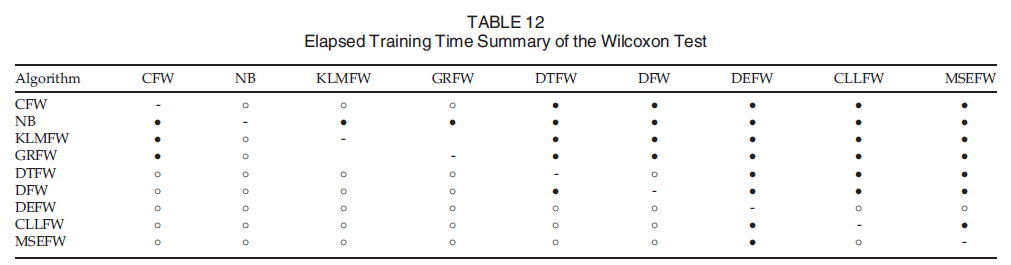
\includegraphics[width=\linewidth]{images/article2/table12.png}
    \caption{}
    \label{a2_table12}
\end{figure}

\clearpage

\begin{figure}
    \centering
    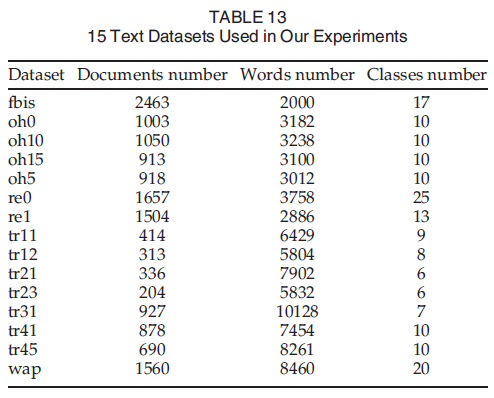
\includegraphics[width=\linewidth]{images/article2/table13.png}
    \caption{}
    \label{a2_table13}
\end{figure}

\begin{figure}
    \centering
    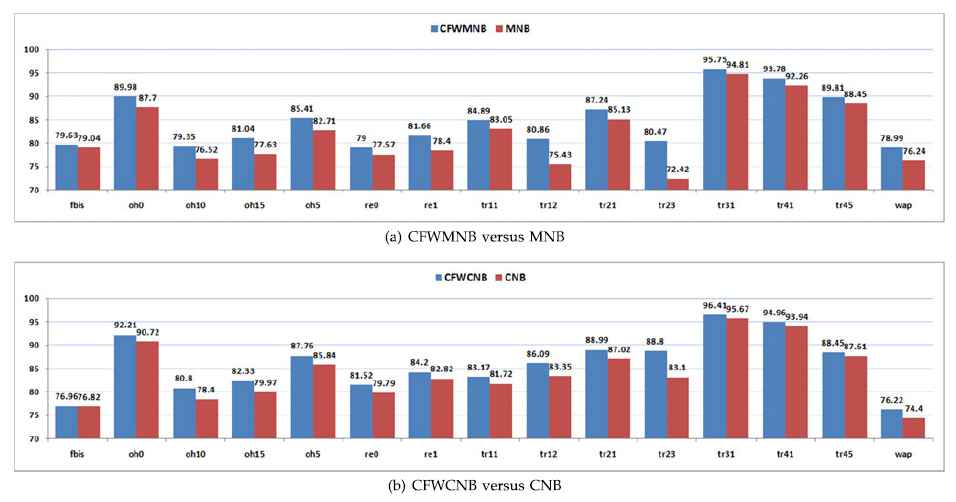
\includegraphics[width=\linewidth]{images/article2/figure.png}
    \caption{}
    \label{a2_figure}
\end{figure}

\clearpage

\section*{مقاله سوم}

در این مقاله، برخلاف مقاله‌های اول و دوم، وزن یک ویژگی در دسته‌های
مختلف یکسان در نظر گرفته نشده است. البته ایده انجام چنین کاری توسط این مقاله
مطرح نشده و پیش‌تر در طی پژوهش‌های مختلف چنین ایده‌ای به کار گرفته شده است.
هنر این مقاله پیشنهاد روش بهتری برای انجام این کار بوده است.

همچنین در مقالات پیشین روش معرفی شده، روشی عام منظوره برای همه مسائل
\lr{naive Bayes} بود. به طور دقیق‌تر، در آن مقاله‌ها ابتدا روش کلی ترسیم می‌شد و
سپس به عنوان یکی از کاربرد‌های مهم، روش معرفی شده بر روی مسائل دسته‌بندی
متن تست می‌شد. اما در این مقاله از همان ابتدا تمرکز مقاله بر دسته‌بندی متن
با استفاده از روش \lr{MNB} بوده و دیگر سایر روش‌های دسته‌بندی متن را بررسی نشده است.
در ادامه جزئیات مقاله بیشتر توضیح داده می‌شود.

\begin{table}[h]
    \centering
    \caption{مشخصات مقاله سوم}
    \label{third_article}
    \begin{tabular}{c|p{.7\linewidth}}
        مشخصه       & توضیح                                                             \\
        \hline
        عنوان مقاله & \lr{Class-Specific Deep Feature Weighting for Naive Bayes Text Classifiers} \\
        سال انتشار  & 2020
    \end{tabular}
\end{table}

\subsection*{روش پیشنهادی}

در این مقاله در ابتدا روش‌های پیشنهاد شده توسط دیگران مرور شده است. با توجه به
اهمیت این روش‌ها در روش ارائه شده توسط این مقاله، این روش‌های مختصرا معرفی و
توضیح داده می‌شوند.

\subsubsection*{وزن‌دهی ویژگی‌ها با استفاده از $\chi^2$}

هدف از محاسبه $\chi^2$ بررسی این فرضیه است که آیا دو متغیر از هم مستقل هستند
یا خیر. برای محاسبه $\chi^2$ جدول مطابق \ref{contingency_table} به نام
\lr{contingency table} ترسیم می‌شود. در این جدول منظور از $w$ یک کلمه
خاص و منظور از $c$ یک دسته خاص است. منظور از $O(w, c)$ نیز تعداد مستنداتی
است که در دسته $c$ قرار داشته و دارای کلمه $w$ بوده‌اند.

\begin{latin}
\begin{table}[h]
    \centering
    \caption{contingency table general form}
    \label{contingency_table}
    \begin{tabular}{c|c|c}
                 & $c$            & $\lnot c$  \\
        \hline
        $w$ & $O(w, c)$ & $O(w, \lnot c)$ \\
        $\lnot w$ & $O(\lnot w, c)$ & $O(\lnot w, \lnot c)$ \\
    \end{tabular}
\end{table}
\end{latin}

پس از به دست آوردن جدول بالا برای هر کلمه و برای هر دسته، مقدار $E(i, j)$
را محاسبه می‌کنیم.

\begin{eqnarray}
    E(i,j) = \frac{\sum_{a \in \{w, \lnot w \}}O(a, j)\sum_{b\in\{c, \lnot c\}}O(i, b)}{n}
\end{eqnarray}

با محاسبه $E(i,j)$ها می‌توانیم مقدار $\chi_{w, c}^2$ را به طریق زیر
برای هر کلمه و هر دسته محاسبه کنیم.

\begin{eqnarray}
    \chi_{w, c}^2 = \sum_{i \in \{w, \lnot w\}}\sum_{j \in \{c, \lnot c\}} \frac{(O(i,j) - E(i,j))^2}{E(i,j)}
\end{eqnarray}

رابطه‌ی بالا را با استفاده از احتمال‌ها می‌توان به شکل زیر بازنویسی کرد.

\begin{eqnarray}
    \chi_{w, c}^2 = \frac{n(p(w, c) p(\lnot w, \lnot c) - p(w, \lnot c) p(\lnot w, c))^2}{p(w)p(\lnot w)p(\lnot c)p(c)}
\end{eqnarray}

همان‌طور که ذکر شد، از معیار $\chi_{w, c}^2$ برای نشان دادن استقلال میان دو
متغیر استفاده می‌شود. بدین طریق که اگر مقدار $\chi_{w, c}^2$ از یک مقداری
کم‌تر باشد می‌توان با اطمینان بیان کرد که دو متغیر مد نظر از هم مستقل هستند و بالعکس.
از این ویژگی $\chi^2$ می‌توان به صورت ضریبی برای بهبود عملکرد
\lr{naive Bayes} استفاده کرد. برای روش وزن‌دهی با استفاده از $\chi^2$
بهبود‌هایی نیز پیشنهاد شده است. برای مثال یکی از پیشنهاد‌ها این است
که جذر $\chi_{w, c}^2$ به عنوان ضریب در نظر گرفته شود.
به عبارت دقیق‌تر آن‌ها معیار پیشنهادی خود را با نام $CC_{w, c}^2$
به شکل زیر معرفی کرده‌اند.

\begin{eqnarray}
    CC_{w, c} = \frac{\sqrt{n}(p(w, c) p(\lnot w, \lnot c) - p(w, \lnot c) p(\lnot w, c))}{\sqrt{p(w)p(\lnot w)p(\lnot c)p(c)}}
\end{eqnarray}

که برابر است با $(CC_{w, c})^2 = \chi_{w, c}^2$.
هدف از ارائه $CC_{w, c}$ تفاوت قائل شدن میان همبستگی مثبت و همبستگی منفی است.
به عبارت بهتر در $\chi_{w, c}^2$ از آن جا که حاصل عبارت زیر به توان دو می‌رسد
بنابراین میان ویژگی‌هایی که این مقدار برای آن‌ها مثبت است و ویژگی‌هایی که
این مقدار برای آن‌ها منفی است نمی‌توان تفکیک قائل شد.

روش وزن‌دهی $\chi^2$ برای دسته‌هایی که تعداد داده کم داشته و
توزیع کلمه در دسته‌ها یکسان نیست، بایاس داشته
و به خوبی عمل نمی‌کند. برای نشان دادن این موضوع از مثال کمک می‌گیریم. در جدول
\ref{where_chi2_fails} جدول \lr{contingency} برای دو کلمه از یک مجموعه داده
را نشان می‌دهد.

طبق جدول $w_1$ نسبت به $w_2$ برای پیش‌بینی بهتر است. $w_2$ علی‌رغم دارا بودن
تعداد رخداد بیشتر نسبت به $w_1$ ($380$ در مقابل $120$)
احتمال وقوع بیشتری نسبت به $w_2$ دارد
($\frac{40}{120}=\frac{1}{3}$ در مقابل $\frac{60}{380}=\frac{3}{19}$).
بعلاوه هر دو کلمه دارای احتمال تقریبا یکسانی هستند که در دسته $c$ باشند.
احتمال این که داده $w_1$ در کلاس $c$ باشد برابر
$\frac{40}{100}=\frac{2}{5}$ و برای کلمه $w_2$ برابر
$\frac{60}{100}=\frac{3}{5}$ است.

با وجود همه‌ی شواهد بالا، معیار $\chi^2$ برای هر دو کلمه مقدار یکسانی را گزارش می‌دهد.
$\chi^2_{w_1, c} = \chi^2_{w_2, c} = 17.61$. به عبارتی
روش $\chi^2$ در راستای پاسخ به این سوال که آیا این دو متغیر به هم وابسته هستند یا نه
پیش رفته و تلاش می‌کند خلاصه‌ی جدول \lr{contingency} را بیان کند و بدین صورت
از میزان همبستگی بین دو متغیر غافل می‌شود. روش بعدی سعی دارد مشکلات این روش
را بهبود داده و از خطاهای این چنینی جلوگیری کند.

\begin{latin}
\begin{table}[t]
    \caption{where $\chi^2$ fails}
    \label{where_chi2_fails}
    \centering
    \hfill
    \begin{tabular}{L|LL|L}
        & c & \lnot c & \Sigma \\
        \hline
        w_1       & 40 & 80 & 120 \\
        \lnot w_1 & 60 & 320 & 380 \\
        \hline
        \Sigma    & 100 & 400 & 500
    \end{tabular}
    \hfill
    \begin{tabular}{L|LL|L}
        & c & \lnot c & \Sigma \\
        \hline
        w_2       & 60 & 320 & 380 \\
        \lnot w_2 & 40 & 80 & 120 \\
        \hline
        \Sigma    & 100 & 400 & 500
    \end{tabular}
    \hfill
\end{table}
\end{latin}

\subsubsection*{وزن دهی با استفاده از روش $R_{w,c}$}

در این روش یک معیار جدید برحسب $O(w, c)$ و $E(w, c)$ به صورت زیر تعریف می‌شود.

\begin{eqnarray}
    R_{w, c} = \frac{O(w, c)}{E(w, c)}
\end{eqnarray}

این معیار را به صورت‌های دیگر نیز می‌توان تعریف کرد.

\begin{eqnarray}
    R_{w, c} & = & \frac{p(w,c)p(\lnot w, \lnot c) - p(w, \lnot c) p(\lnot w, c)}{p(w)p(c)} + 1 \\
    R_{w, c} & = & \frac{p(w|c)}{p(w)}
\end{eqnarray}

اگر این معیار را برای جدول \ref{where_chi2_fails} محاسبه کنیم، درستی عملکرد
این معیار را مشاهده می‌کنیم.

\begin{eqnarray*}
    R_{w_1, c} & = & \frac{40}{500} \times (\frac{100}{500})^{-1} \times (\frac{120}{500})^{-1} = 1.67 \\
    R_{w_2, c} & = & \frac{60}{500} \times (\frac{100}{500})^{-1} \times (\frac{380}{500})^{-1} = 0.78
\end{eqnarray*}

همان‌طور که مشاهده می‌شود، عدد برگردانده شده توسط معیار $R_{w, c}$ برای هر یک از
کلمات متفاوت است.

در روش پیشنهادی برای وزن‌دهی لزوما $W_{w,c} = R_{w, c}$ نیست.
از رابطه‌ی زیر برای تبدیل $R_{w,c}$
به $W_{w, c}$ استفاده می‌شود.

\begin{eqnarray}
    W_{w, c} =
    \begin{cases}
        R_{w, c} & R_{w, c} > 1 \\
        1 & R_{w,c} \leq 1
    \end{cases}
\end{eqnarray}

روش $R_{w,c}$ نیز خالی از اشکال نیست. برای مثال جدول \ref{where_R_fails}
را در نظر بگیرید.

\begin{latin}
    \begin{table}[h]
        \centering
        \caption{where $R_{w, c}$ fails}
        \label{where_R_fails}
        \begin{tabular}{L|LLL|L}
            & c_1 & c_2 & c_3 & \Sigma \\
            \hline
            w_1 & 1 & 20 & 20 & 41 \\
            w_2 & 0 & 1 & 20 & 21 \\
            w_3 & 0 & 0 & 1 & 1\\
            \hline
            \Sigma & 1 & 21 & 41 & 63
        \end{tabular}
    \end{table}
\end{latin}

با محاسبه $R_{w_1, c_1}$ و $R_{w_1, c_2}$ داریم.

\begin{eqnarray*}
    R_{w_1, c_1} & = & \frac{1/1}{41/63} = 1.536 \\
    R_{w_1, c_2} & = & \frac{20/21}{41/63} = 1.463
\end{eqnarray*}

مقدار $R_{w_1, c_1} > R_{w_1, c_2}$ است. و این بدین معنی است که
کلمه $w_1$ به کلاس $c_1$ مربوط‌تر است.
در حالی که آمار موجود در جدول \ref{where_R_fails} عکس این مطلب را بیان می‌کند. مطابق
جدول \ref{where_R_fails} تنها $\frac{1}{41}$ از مستنداتی که حاوی $w_1$ هستند
در کلاس $c_1$ قرار دارند. در حالی که $\frac{20}{41}$ از مستنداتی که حاوی
کلمه $w_1$ هستند در دسته $c_2$ قرار دارند. روش بعدی که روش معرفی شده در مقاله
\lr{Class-Specific Deep Feature Weighting for Naive Bayes Text Classifiers}
است به حل این مسئله می‌پردازد.

\subsubsection*{روش $CR_{w, c}$}

در این روش چهار مشخصه برای بررسی
ارتباط بین کلاس $c$ و کلمه $w$ در نظر گرفته می‌شود.

\begin{itemize}
    \item $P(w)$: توزیع کلمه $w$ در کل داده‌های آموزشی
    \item $P(w|c)$: توزیع کلمه $w$ در داده‌های با برچسب $c$
    \item $P(c|w)$: توزیع مستندات شامل کلمه $w$ در بین کلاس‌های مختلف
    \item تعداد برچسب‌های مختلف مستند شامل کلمه $w$
\end{itemize}

روش $R_{w,c}$ تنها دو معیار اول را مورد توجه قرار می‌داد و
به همین دلیل در مثال جدول \ref{where_R_fails} نمی‌توانست به خوبی عمل کند.
بر این اساس $CR_{w,c}$ سعی می‌کند با دخیل کردن دو مشخصه دیگر معیار $R_{w,c}$
را بهبود ببخشد. $CR_{w,c}$ بر اساس $R_{w,c}$ به شکل زیر تعریف می‌شود.

\begin{eqnarray}
    CR_{w, c} & = & R_{w, c} \frac{P(w, c)}{P(w)} \ln(2 + \frac{n_c}{k_w})
\end{eqnarray}

با صرف نظر از نماد‌هایی که قبل‌تر معرفی شده است، نماد $n_c$ نشان‌دهنده تعداد کل
دسته‌ها و $k_w$ نشان دهنده تعداد دسته‌های مستندات شامل کلمه $w$ است.

برای مقایسه عملکرد $CR_{w,c}$ با $R_{w,c}$ محاسبات انجام شده برای جدول \ref{where_R_fails}
را با $CR_{w,c}$ تکرار می‌کنیم.

\begin{eqnarray}
    CR_{w_1, c_1} & = & 1.536 \times \frac{\frac{1}{63}}{\frac{41}{63}} \times \ln(2+\frac{3}{3}) = 0.412 \\
    CR_{w_1, c_2} & = & 1.463 \times \frac{\frac{20}{63}}{\frac{41}{63}} \times \ln(2+\frac{3}{3}) = 0.784
\end{eqnarray}

همان‌طور که مشاهده می‌شود، معیار $CR_{w,c}$ به درستی برای کلمه $w_1$ در کلاس $c_1$
عدد کمتری نسبت به همین کلمه در کلاس $c_2$ نسبت داد.

پس از محاسبه $CR_{w,c}$برای $w$ها و $c$های مختلف، مقادیر $CR_{w,c}$ها به
عنوان $W_{w,c}$ در نظر گرفته می‌شود. همچنین در این مقاله از فرمول‌های زیر
برای دسته‌بندی داده‌ها استفاده می‌شود.

\begin{eqnarray}
    P(c) & = & \frac{\sum_{j=1}^{n}\delta(c_j, c) + 1}{n+n_c} \\
    P(w_i|c) & = & \frac{\sum_{j=1}^{n} CR_{w_i,c}f_{ji}\delta(c_j, c) + 1}{\sum_{i=1}^{m}\sum_{j=1}^{n} CR_{w_i,c} f_{ji}\delta(c_j,c)+m} \\
    c(d) & = & \argmax_{c \in C} \Bigl(\log P(c) + \sum_{i=1}^{m} CR_{w_i,c} f_i \log P(w_i| c)\Bigr)
\end{eqnarray}

با اندکی دقت در این فرمول‌ها مشخص می‌شود که این فرمول‌ها همان فرمول‌های استفاده شده
در مقاله اول است.

\clearpage

\subsection*{نتایج}

نتایج اجرای روش ارائه شده در مقاله با روش‌های پیشین ارائه شده در شکل‌های
\ref{a3_table8} و \ref{a3_results} دیده می‌شود.

\begin{figure}[h]
    \centering
    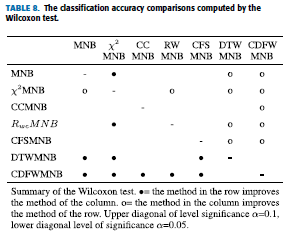
\includegraphics[scale=0.7]{images/article3/table8.png}
    \caption{}
    \label{a3_table8}
\end{figure}

در ابتدا نیاز است تا نام کامل سایر روش‌ها ارائه شود.

\begin{itemize}
    \item \lr{MNB}: روش بیز ساده چندجمله
    \item \lr{$\chi^2$ MNB}: روش بیز ساده چندجمله‌ای با وزن دهی $\chi^2$
    \item \lr{$CC$ MNB}: روش بیز ساده چندجمله‌ای با وزن دهی $CC$
    \item \lr{$R_{w,c}$ MNB}: روش بیز ساده چندجمله‌ای با وزن دهی $R_{w,c}$
    \item \lr{CFSMNB}: روش بیز ساده با وزن‌دهی مبتنی بر روش \lr{CFS} (این روش
          همان روش ارائه شده در مقاله اول است.)
    \item \lr{DRWMNB}: روش بیز ساده چندجمله‌ای با وزن‌های مبتنی بر ساخت درخت
    \item \lr{CDFWMNB}: روش ارائه شده در این مقاله
\end{itemize}

همان‌طور که مشاهده می‌شود، نتایج روش این مقاله با روش ارائه شده توسط مقاله اول
بررسی شده اما با روش ارائه شده در مقاله دوم بررسی نشده است. این موضوع عجیب
بوده و این شبهه را ایجاد می‌کند که آیا نتایج عملکرد این روش از نتایج روش
مقاله دوم بهتر است یا بد‌تر؟

برای انجام تست‌ها از محیط \lr{Weka} استفاده شده است. برای ارائه نتایج،
هر دیتاست به ۱۰ بخش تقسیم شده و هر بار با ۹ قسمت آن آموزش صورت گرفته
و با تکه ۱۰‌ام آن ارزیابی صورت گرفته است. همچنین این عمل تکه‌تکه کردن دیتاست
۱۰ بار برای هر دیتاست انجام شده است.

نکات زیر در نتایج مهم به نظر می‌رسد.

\begin{itemize}
    \item شکل \ref{a3_table5} مجموعه دادگان استفاده شده را نشان می‌دهد.
          تعداد مجموعه‌های استفاده شده برای مطمئن بودن از نتایج مناسب بوده و همچنین
          به دلیل دسترسی عمومی به این دیتاست‌ها و معروف بودن آن‌ها نتایج قابل تکرار است.
    \item در شکل \ref{a3_table6} صحت عملکرد روش‌های مختلف آورده شده است. همان‌طور
          که مشاهده می‌شود بهترین میانگین صحت با اختلاف چند درصدی، برای روش ارائه شده
          در این مقاله است. اما نویسندگان تنها به وجود این اختلاف بسنده نکرده‌اند
          و برای نشان ‌دادن آن که نتایج روش خود با باقی روش‌ها متفاوت است از تست
          \lr{Friedman} کمک گرفته‌اند. این تست نیز اختلاف نتایج با درصد اطمینان 95 درصد
          را گزارش کرده است.
    \item در ادامه نویسندگان با استفاده از تست \lr{Post-hoc Holm} و
          \lr{wilcoxon} عملکرد روش‌ها را دوبه‌دوی بررسی کرده‌اند. این روش‌ها نیز
          عملکرد ممتاز روش ارائه شده را تایید کرده‌اند.
    \item در نهایت محققان به سراغ تست سرعت یادگیری روش خود پرداخته‌اند.
          نتایج این تست نیز که در شکل \ref{a3_table9} دیده می‌شود، عملکرد ممتاز
          این روش را تایید می‌کند. نکته جالبی که در این جدول وجود دارد عملکرد بسیار
          ضعیف روش \lr{CFSMNB} است که برای آموزش به ۱۰۰ واحد زمانی نیاز دارد.
          این در حالی است که این روش وزن یکسانی برای یک ویژگی‌ در دسته‌های مختلف
          در نظر می‌گیرد در حالی که روش \lr{CDFWMNB} برای هر ویژگی در
          هر کلاس یک وزن اختصاص می‌دهد.
    \item نکته‌ای که از نظر نویسندگان مغفول مانده است مقایسه روش‌ها از نظر
          میزان حافظه مصرفی است. چرا که بسیار محتمل است پیاده‌سازی یک روش به صورتی انجام
          گیرد که با وجود سریع بودن حافظه بسیاری را اشغال کند.
\end{itemize}

\begin{figure}
    \begin{subfigure}{0.45\linewidth}
        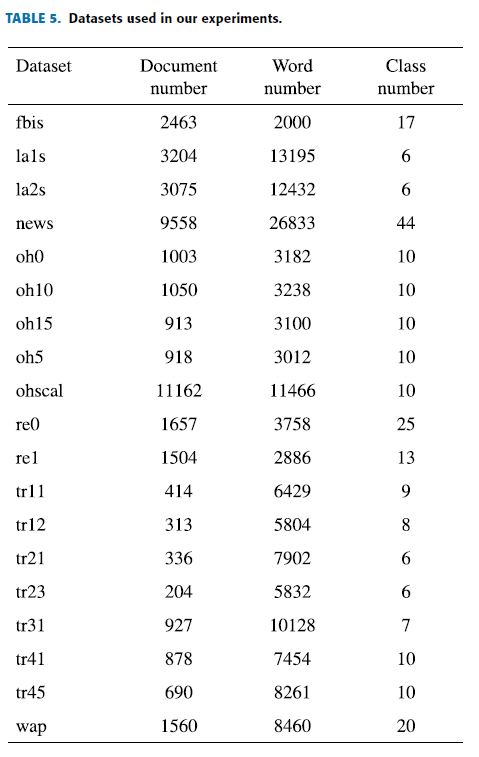
\includegraphics[width=\linewidth]{images/article3/table5.png}
        \caption{}
        \label{a3_table5}
    \end{subfigure}
    \hfill
    \begin{subfigure}{0.45\linewidth}
        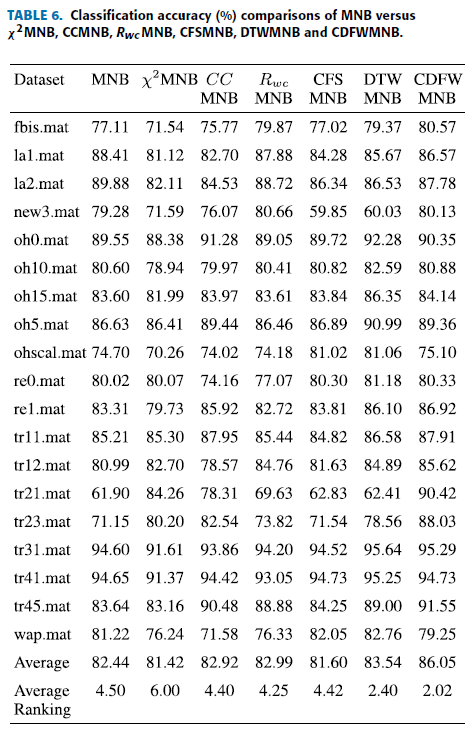
\includegraphics[width=\linewidth]{images/article3/table6.png}
        \caption{}
        \label{a3_table6}
    \end{subfigure}
    \newline
    \begin{subfigure}{0.45\linewidth}
        \centering
        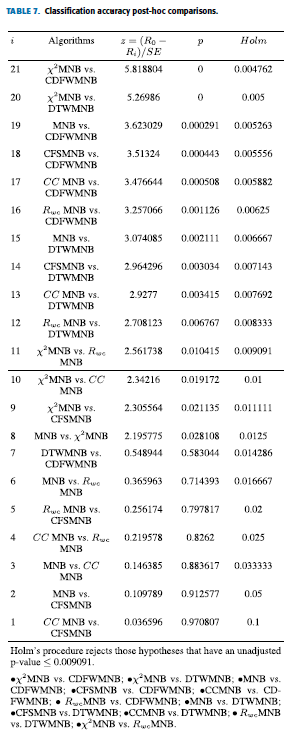
\includegraphics[scale=0.55]{images/article3/table7.png}
        \caption{}
        \label{a3_table7}
    \end{subfigure}
    \hfill
    \begin{subfigure}{0.45\linewidth}
        \centering
        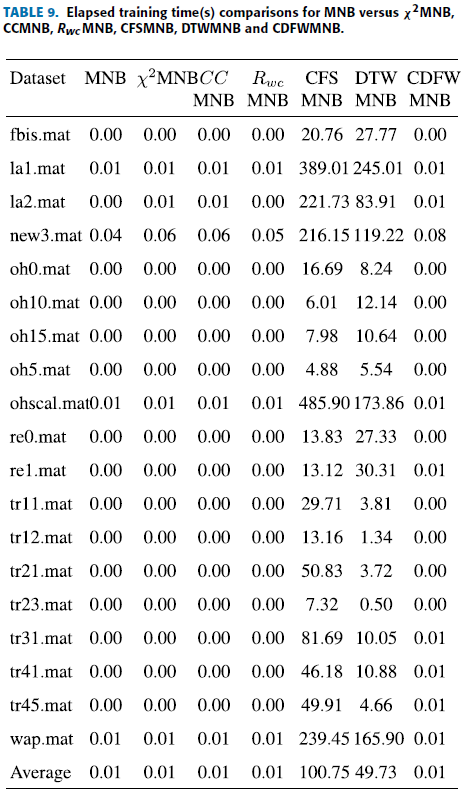
\includegraphics[width=\linewidth]{images/article3/table9.png}
        \caption{}
        \label{a3_table9}
    \end{subfigure}
    \caption{نتایج گزارش شده مقاله سوم}
    \label{a3_results}
\end{figure}

\end{document}